\documentclass[titlepage=true]{scrartcl}

\usepackage{preamble}

\begin{document}

\SSfp

\section*{Introduction} 
\addcontentsline{toc}{section}{Introduction}
    Welcome to the OpenPOTD solutions booklet! Here you'll find answers \& solutions to all past seasons.\medskip

Solutions for season one were entirely written up by {\fontfamily{qcr}\selectfont Brainysmurfs\#2860}, while {\fontfamily{qcr}\selectfont .19\#9839} has overseen most of season two. 
From season three onwards, Yuchan ({\fontfamily{qcr}\selectfont Angry Any\#4319}) has also been contributing problem proposals and solutions. 

Where possible, from season two onwards, We have tried to include the officially provided solutions to problems, 
or adapted them in line with any changes to the problem statement, and in most cases also and filled in the gaps as best I could, 
to make solutions more approachable to beginners. 
For the more well known questions that are featured in a season (namely problems from the International Mathematical Olympiad), 
instead of providing our own solution, we have included the \emph{Art of Problem Solving} forum post on the question, 
which will contain multiple solution write-ups, as well as discussion about the problem.

In many circumstances problems have not come with official write-ups - or indeed write-ups of any kind - 
and thus have required us to provide our own. In these cases we humbly apologise for any mistakes (or fakesolves!) in advance. 
If you do notice any mistakes, check out How to contribute.\medskip

\addcontentsline{toc}{subsection}{How to Contribute}
\subsection*{How to Contribute}
\label{sec:contribute}

If you would like to contribute to the project - be that through correcting a mistake in the document, 
wanting to contribute a solution write up - or even proposing a problem for a future season, here's how.\medskip

\addcontentsline{toc}{subsubsection}{Correcting Mistakes}
\subsubsection*{Correcting Mistakes}
\label{sec:mistakes}

If you notice any mistakes while going through the solutions document, be it a typo or missing or incorrect information about a particular problem, feel free to submit a push request with the fix. 
If you don't feel comfortable doing that, you can always contact us (see the \hyperref[sec:contact]{Contact Us} to find out how), 
and we'll be happy to fix the error. Alternatively, you can open up an \href{https://github.com/OpenPOTD/Solutions/issues}{Issue} on the GitHub, or mention it in the \href{https://github.com/OpenPOTD/Solutions/discussions}{discussions tab}.\medskip

\addcontentsline{toc}{subsubsection}{Contributing Solutions}
\subsubsection*{Contributing Solutions}
\label{sec:solutions}

Similarly to correcting any mistakes, if you would like to contribute a write-up to a particular problem, 
you can submit a push containing the solution - doing as Romans do (i.e. just look at how others have submitted write-ups and copy that). 
If you are submitting a push, make sure you edit {\fontfamily{qcr}\selectfont preamble.sty} to include your Discord information in a macro 
(scroll to the bottom of the file and you'll see), so that you can include yourself in the contributors list. 
Furthermore, make sure that you credit your solution with {\fontfamily{qcr}\selectfont[Write up by ...]}. 
If any of that sounds complicated or you forget to add that information, that's fine - we'll add it for you.

If creating push requests and fiddling with LaTeX isn't your thing, we'll gladly help you type it up
 if you write it out in plaintext or whatever medium you feel most comfortable using (so long as we can understand it!) - 
 to do this just send it to us using any of the options in \hyperref[sec:contact]{Contact Us}. 
 Similarly, you can use the GitHub \href{https://github.com/OpenPOTD/Solutions/discussions}{discussions tab} and post it there.\medskip 

\textbf{\emph{Note: feel free to submit alternative solutions to any past problems, be it from season 1, or the most recent}}\medskip

\addcontentsline{toc}{subsubsection}{Problem Proposals}
\subsubsection*{Problem Proposals}
\label{sec:problems}

If you'd like to submit a problem proposal - be it an original problem, or just a particular problem you found interesting - 
we're always on the lookout for new problems! For original problems, please ensure you submit the problem with a solution. 
As with solution write-ups, though sending us a {\fontfamily{qcr}\selectfont .tex} file is preferred, it's completely fine to just send a plaintext write up, or a screenshot etc. 
and we can deal with it from there. The same goes for non-original problems, though solutions aren't required, 
they would be greatly appreciated. If you are submitting a non-original problem please ensure you include the problem source. 

Please do not use a public medium to submit a problem proposal - messaging one of us on Discord would
 be the preferred method of communication (See \hyperref[sec:contact]{Contact Us}).\medskip

\addcontentsline{toc}{subsubsection}{Feature Suggestions}
\subsubsection*{Feature Suggestions} 
\label{sec:suggestions}

If you have any ideas when it comes to improving the bot or project, the best place to do that is in the {\fontfamily{qcr}\selectfont \#Suggestions} channel, or any of the other methods listed in \hyperref[sec:contact]{Contact Us}, such as using the GitHub \href{https://github.com/OpenPOTD/Solutions/discussions}{discussions tab}.\medskip

\addcontentsline{toc}{subsection}{Contact Us}
\subsection*{Contact Us}
\label{sec:contact} 

The best way to contact us is through the \href{https://discord.gg/GsPSSHdhPB}{OpenPOTD Discord server}, 
however, you may also contact us through the \href{https://github.com/OpenPOTD/Solutions/discussions}{discussions tab} on Github.
 Alternatively, you can DM any of us on Discord:

 \begin{itemize}
     \item .19\#9839 (434767660182405131)
     \item brainysmurfs\#2860 (281300961312374785)
     \item Angry Any\#4319 (580933385090891797)
 \end{itemize}
 \medskip

\addcontentsline{toc}{subsection}{Contributors}
\subsection*{Contributors}
\label{sec:contributors}

Thank you (in no particular order) to the following contributors:
\footnote{The numbers are in the format: Season.Week.Problem}\medskip

\Paiya: Solution write-ups (\hyperref[2-1-1]{2.1.1}, \hyperref[2-1-3]{2.1.3}, \hyperref[2-1-4]{2.1.4})\\
\Ptony: Original problem proposal (\hyperref[1-1-2]{1.1.2})\\
\Ppi: Original problem proposal (\hyperref[1-1-6]{1.1.6}, \hyperref[1-2-5]{1.2.5})\\
\Pbfan: Original problem proposal (\hyperref[1-1-7]{1.1.7})\\
\Pkiesh: Original problem proposal (\hyperref[1-2-3]{1.2.3})\\
\Pchris: Problem proposal (\hyperref[2-1-6]{2.1.6})\\
\Pkee: Original problem proposal (\hyperref[2-2-3]{2.2.3})\\
\PSlas: Solution write-up (\hyperref[2-2-5]{2.2.5})\\
\Parjun: Typo fixes
\newpage

\pagenumbering{arabic}

\ihead{\footnotesize\bfseries\sffamily{Season 1, Week 1}}
\section{Season 1}

    \subsection{Week 1}
        
        \subsubsection{Intersecting Circles}
            \label{1-1-1}
            \SSbreak\\
\emph{Source: \Csmc, 2015 Q4}\\
\emph{Proposer: \Pbrain}\\
\emph{Problem ID: 21}\\
\emph{Date: 2020-10-27}\\
\SSbreak

\SSpsetQ{
    Consider the positive integer \(N\), and Two internally tangent circles \( \Gamma_1 \) and \( \Gamma_2 \) 
    are given such that \( \Gamma_1 \) passes through the center of \( \Gamma_2 \). 
    Find the fraction of the area of \( \Gamma_1 \) lying outside \( \Gamma_2 \). 
    If this fraction is \( \frac ab \) where \( \gcd(a, b) = 1\), then find \( a+b \).
}\bigskip

\begin{solution}\hfil\medskip

    Suppose $\Gamma_2$ has radius $2r$. Since $\Gamma_1$ is internally tangent to $\Gamma_2$ and passes through its centre, the radius of $\Gamma_1$ is half the radius of $\Gamma_2$, 
    i.e. just $r$. So fraction of the area of $\Gamma_1$ lying outside $\Gamma_2$ is $\dfrac{4\pi r^2 - \pi r^2}{4 \pi r^2} = \dfrac{3}{4}$. 
    Since $3 + 4 = 7$, the answer is $\boxed{7}$
\end{solution}\bigskip
        \newpage

        \subsubsection{Guava Juice}
            \label{1-1-2}
            \SSbreak\\
\emph{Source: \Cop}\\
\emph{Proposer: \Ptony}\\
\emph{Problem ID: 22}\\
\emph{Date: 2020-10-28}\\
\SSbreak

\SSpsetQ{
    The ingredients list of a Guava Juice Drink is as follows:
        \begin{quote}
            Water (80\%), Guava Juice, Sugar, Fructose (3\%), Sodium Carboxymethyl Cellulose, Citric Acid, Flavour, Vitamin C (0.04\%)
        \end{quote}
    Assuming only that the ingredients list is ordered by their constituent percentage in the drink (which are not necessarily distinct), 
    find the maximum and minimum possible percentage of Guava Juice in the drink. If their difference is \(n\), submit \(100n\).
}\bigskip

\begin{solution}\hfil\medskip

    Note there are 2 ingredients between water and fructose, and 3 between fructose and Vitamin C. \\

    For the amount of guava juice to be maximised, everything should be minimised. 
    In particular, there should be 0.04\% of Sodium Carboxymethyl Cellulose, Citric Acid, and Flavour; and 3\% of Sugar and Fructose. 
    This gives us a Guava Juice percentage of 13.84\%. \\

    For the amount of guava juice to be minimised, everything else should be maximised. 
    In particular, there should be 3\% of Sodium Carboxymethyl Cellulose, Citric Acid, and Flavour;
     and equal amounts of sugar and guava juice. 
    This gives us a guava juice percentage of 5.48\%. \\

    This gives us $13.84 - 3.98 = 9.86 \%$. 
    Multiplying this by $100$ gives us $\boxed{986}$. 
\end{solution}\bigskip
        \newpage 

        \subsubsection{Complex Roots}
            \label{1-1-3}
            \SSbreak\\
\emph{Source: New South Wales Higher School Certificate `4U', 2020 Q2}\\
\emph{Proposer: \Pbrain}\\
\emph{Problem ID: 23}\\
\emph{Date: 2020-10-29}\\
\SSbreak

\SSpsetQ{
    Given that \( z = 3+i \) is a root of \( z^2+pz+q=0 \), where \( p \) and \( q \) are real, 
    find the values of \(p\) and \(q\), and submit \( p+q \).
}\bigskip

\begin{solution}\hfil\medskip
    
    Applying the Complex Conjugate Theorem, $z=3  i$ is also a root of the quadratic. 
    Expanding $(z-3-i)(z-3+i)$ gives us $z^2-6z+10$. Thus $p = -6$ and $q = 10$, meaning $p + q = \boxed{4}$.
\end{solution}\bigskip
        \newpage 

        \subsubsection{Exponents}
            \label{1-1-4}
            \SSbreak\\
\emph{Source: \Csmo Junior Round 1, 2001 Q4}\\
\emph{Proposer: \Pbrain}\\
\emph{Problem ID: 25}\\
\emph{Date: 2020-10-30}\\
\SSbreak

\SSpsetQ{
    If \( a \) and \( b \) are positive reals such that \( a^b = b^a \) and \( b = 2a \), 
    then the value of \( b^2 \) is? 
}\bigskip

\begin{solution}\hfil\medskip

    A direct search yields that $2^4 = 4^2$ and $4 = 2 \times 2$. 
    The problem implies that such a unique value for $b$ exists, hence $b^2 = \boxed{16}$.
\end{solution}\bigskip
        \newpage

        \subsubsection{Volumes of Cubes}
            \label{1-1-5}
            \SSbreak\\
\emph{Source: \Cnzsmc Round 2, 2019 Q7}\\
\emph{Proposer: \Pbrain}\\
\emph{Problem ID: 26}\\
\emph{Date: 2020-10-31}\\
\SSbreak

\SSpsetQ{
    Two cubes with positive integer side lengths are such that the sum of their volumes is numerically equal to the difference of their surface areas. Find the sum of their volumes.
}\bigskip 

\begin{solution}\hfil\medskip 

    A direct search yields that cubes of side length $4$ and $2$ satisfy the condition. The answer is thus $4^3 + 2^3 = \boxed{72}$.
\end{solution}\bigskip
        \newpage

        \subsubsection{Complex Mess}
            \label{1-1-6}
            \SSbreak\\
\emph{Source: \Cop}\\
\emph{Proposer: \Ppi}\\
\emph{Problem ID: 24}\\
\emph{Date: 2020-11-01}\\
\SSbreak

\SSpsetQ{
    Suppose \[ \left ( \sqrt{5} + i\sqrt{10-2\sqrt{5}} + 1 \right )^{2020} = a^b \] for some
     \( a, b \in \Z \) where \( b \) is maximised. Compute \( a+b \).
}\bigskip

\begin{solution}\hfil\medskip
    
    Notice that $ \left ( \sqrt{5} + i\sqrt{10-2\sqrt{5}} + 1 \right ) = 4 \mathrm{cis} \frac{\pi}{5}$. 
    In particular, by De Moirve's Theorem, 
    $$\left ( \sqrt{5} + i\sqrt{10-2\sqrt{5}} + 1 \right )^{2020} = 4^{2020} \mathrm{cis} {404\pi} = 2^{4040}$$.\\

    So the answer is $2 + 4040 = \boxed{4042}$. 
\end{solution}\bigskip
        \newpage 

        \subsubsection{Paper Eating}
            \label{1-1-7}
            \SSbreak\\ 
\emph{Source: \Cop}\\
\emph{Proposer: \Pbfan}\\
\emph{Problem ID: 31}\\
\emph{Date: 2020-11-02}\\
\SSbreak

\SSpsetQ{
    Tan and Wen are writing questions for CCCC at a rate of 1 per minute. Immediately after Tan
     writes a question, Wen eats his paper with probability \( \frac 17 \), so that Tan must restart.\\

    After an extremely long time (assume infinite), Tony Wang walks in.
     What is the expected number of questions Tony Wang sees written on Tan's paper?
}\bigskip 

\begin{solution}\hfil\medskip

    Let $E_n$ be the expected number of questions Tony Wang sees written on Tan's paper after $n$ minutes. \\

    Then the following recurrence holds: 
    \[E_{n+1} = \frac{6}{7} (E_n+1) + \frac{1}{7} \cdot 0\]
    because with $\frac{6}{7}$ probability, Tan writes another question without Wen eating it, 
    and with $\frac{1}{7}$ probability, Wen eats all of Tan's questions. \\

    Claim 1: $E_n < 6 ~\forall n$. 

    \begin{subproof}
        The proof is by induction. Note $E_0 = 0$. If $E_k < 6$, then 
        $E_{k+1} = \frac{6}{7} (E_k + 1) < \frac{6}{7} (6 + 1) = 6$. 
        This completes the proof. 
    \end{subproof}

    Claim 2: $E_{n+1} > E_n ~\forall n$. 

    \begin{subproof}
        Note that since $E_k < 6 ~\forall k$, we have 
        $E_{k+1} = \frac{6}{7} (E_k+1) > \frac{6}{7} (E_k + \frac16 E_k) = E_k$. 
    \end{subproof}

    Now by the Monotone Bounded Convergence Theorem, the sequence $\left( E_n \right )$ converges to a limit. 
    Suppose $\lim E_n = L$. Then note $\lim E_{n+1} = L$ since changing the first terms of a sequence does not change the overall convergence. 
    So since $E_{n+1} = \frac{6}{7} (E_n + 1)$, $\lim E_{n+1} = \lim \frac{6}{7} (E_n+1)$. 
    So $L = \frac{6}{7}(L + 1)$. \\

    Solving this, we obtain $L = \boxed{6}$. 
\end{solution}\bigskip
        \newpage
        
\ihead{\footnotesize\bfseries\sffamily{Season 1, Week 2}}
    \subsection{Week 2}

        \subsubsection{Regenerative Watermelons}
            \label{1-2-1}
            \SSbreak\\
\emph{Source: \Cbmoo 2018 Q2}\\
\emph{Proposer: \Pss}\\
\emph{Problem ID: 22}\\
\emph{Date: 2020-11-03}\\
\SSbreak

\SSpsetQ{
    Out of 100 regenerative watermelons, each of six friends eats exactly 75 watermelons. 
    There are \( n \) watermelons eaten by at least five of the friends. 
    What is the sum of the largest and smallest possible values of \( n \)?\\

    \textit{Note: The watermelons are regenerative to allow multiple people to eat the same watermelon. 
    (But the same person cannot eat the same watermelon more than once)}
}\bigskip

\begin{solution}\hfil\medskip

    Maximum: The maximum is 90. Take the sum over all watermelons of how many times they were eaten. 
    This is 450, since all $6 \cdot 75 = 450$. Then since $5n \leq 450$, $n \leq 90$. T
    he construction for the maximum is: staff member $k$ ($k = 1, 2, \cdots, 6$) eats all watermelons from 1 to 90 except those $k \pmod6$. \\

    Minimum: The minimum is 25. We intuit that in the minimum case all the watermelons were either eaten 6 times or 4. 
    Then $6a + 4b = 450$, and $a + b = 75$. Solving yields $a = 25$ and $b = 75$. \\

    The answer is $25 + 90 = \boxed{115}$. 
\end{solution}\bigskip

        \newpage 

        \subsubsection{Largest Prime Factor}
            \label{1-2-2}       
            \SSbreak\\
\emph{Source: \Csmc, 2015 Q23}\\
\emph{Proposer: Unknown}\\
\emph{Problem ID: 27}\\
\emph{Date: 2020-11-04}\\
\SSbreak

\SSpsetQ{
    Given four different non-zero digits, it is possible to form 24 different numbers containing each of these four digits. 
    What is the largest prime factor of the sum of the 24 numbers?
}\bigskip

\begin{solution}\hfil\medskip 

    Say the digits are $a$, $b$, $c$, and $d$. For each digit, it appears in the units place 6 times,
     the tens place 6 times, the hundreds place 6 times, and the thousands place 6 times. \\

    Hence the sum of the 24 numbers is $6666(a+b+c+d) = 2 \cdot 3 \cdot 11 \cdot 101 (a+b+c+d)$.
     Since $a+b+c+d < 40$, it cannot have any prime factors larger than 101. \\

    The largest prime factor of the sum of the 24 numbers is thus $\boxed{101}$. 
\end{solution}\bigskip
        \newpage

        \subsubsection{Real Roots}
            \label{1-2-3}
            \SSbreak\\
\emph{Source: \Cop}\\
\emph{Proposer: \Pkiesh}\\
\emph{Problem ID: 28}\\
\emph{Date: 2020-11-05}\\
\SSbreak

\SSpsetQ{
    If the polynomial \( x^2 + bx + 101 = 0 \) has integer roots \( m \) and \( n \), where 
    \( \vert m \vert > \vert n \vert \), then what is the sum of the positive integer divisors of \( \frac mn \)?
}\bigskip 

\begin{solution}\hfil\medskip 

    By Vieta's Formula $101 = mn$. Since $101$ is prime, $m, n = \pm 101, \pm 1$. So $\frac mn = \pm 101$. 
    The positive divisors of $\pm 101$ are 1 and 101, so their sum is $1 + 101 = \boxed{102}$.
\end{solution}\bigskip

        \newpage 

        \subsubsection{The Meme factor}
            \label{1-2-4}
            \SSbreak\\
\emph{Source: \Cop}\\
\emph{Proposer:  \Pchan}\\
\emph{Problem ID: 32}\\
\emph{Date: 2020-11-06}\\
\SSbreak

\SSpsetQ{
    What is the sum of all integers \( x \) such that \( \frac {6969}x \) is an integer?
}\bigskip 

\begin{solution}\hfil\medskip

    Note that if $\frac{6969}x$ is an integer, so is $\frac{6969}{-x}$. So the sum is $\boxed{0}$.
\end{solution}\bigskip
        \newpage

        \subsubsection{Human Wolfram}
            \label{1-2-5}
            \SSbreak\\
\emph{Source: \Cop}\\
\emph{Proposer: \Ppi}\\
\emph{Problem ID: 33}\\
\emph{Date: 2020-11-07}\\
\SSbreak

\SSpsetQ{
    Compute the number between \(1000\) and \(2000\) that divides \[69^{69} - 5^{69} + 6^{69}.\]
}\bigskip

\begin{solution}\hfil\medskip

    Let $N = 69^{69} - 5^{69} + 6^{69}$. \\
    
    Claim 1: $64 \mid N$. 
    
    \begin{subproof}
        Note that $69 \equiv 5 \pmod{64} \Rightarrow 69^{69} \equiv 5^{69} \pmod{64}$. 
        Further, $6^{69}=64\cdot3^{6}\cdot6^{63}$. So $64 \mid N$. 
    \end{subproof}

    Claim 2: $25 \mid N$.

    \begin{subproof}
        Note that $69 \equiv (-6) \pmod{25} \Rightarrow 69^{69} \equiv (-6)^{69} \pmod{25}$, 
        since 69 is odd. Thus $25 \mid N$ as required. 
    \end{subproof}

    Since $64 \cdot 25 = 1600$ and the question implies there is only one answer, 
    we obtain that the required number is $\boxed{1600}$. 
\end{solution}\bigskip
        \newpage 

        \subsubsection{Guess the Config}
            \label{1-2-6}
            \SSbreak\\
\emph{Source: \Cbmot 2008 Q2}\\
\emph{Proposer: \Pss}\\
\emph{Problem ID: 34}\\
\emph{Date: 2020-11-08}\\
\SSbreak

\SSpsetQ{
    Let triangle \(ABC\) have incentre \(I\) and circumcenter \(O\). 
    Suppose that \( \angle AIO = 90^{\circ} \) and \( \angle CIO = 45^{\circ} \). 
    Suppose the ratio \( AB : BC : CA \) can be expressed as \( a : b : c \) where \( \gcd(a, b, c) = 1 \). 
    Find \( a + b + c \).
}\bigskip 

\begin{solution}\hfil\medskip

    Place a $3-4-5$ triangle on the coordinate plane with $A = (3, 0)$, $B = (0, 0)$ and $C = (0, 4)$. 
    We can compute that $I = (1, 1)$ and $O = (1.5, 2)$. 
    This arrangement of points satisfies the question's constraints, and so the answer is $3 + 4 + 5 = \boxed{12}$. 
\end{solution}\bigskip
        \newpage 
        
        \subsubsection{A Quadratic Mess}
            \label{1-2-7}
            \SSbreak\\
\emph{Source: \Csmo, Open Section Round 2, 2004 Q2}\\
\emph{Proposer: \Pbrain}\\
\emph{Problem ID: 35}\\
\emph{Date: 2020-11-09}\\
\SSbreak

\SSpsetQ{
    Find the number of ordered pairs \( (a, b) \) of integers, where \( 1 \leq a, b \leq 2004 \), 
    such that \[ x^2+ax+b = 167y \] has integer solutions in \( x \) and \( y \).\\
    
    \textit{Note: You are allowed a four-function calculator. }
}\bigskip

\begin{solution}\hfil\medskip 

    Note that 167 is prime. So 
    
    \begin{align*}
        x^2 + ax + b &\equiv 0 \pmod{167} \\
        \iff (x + \frac a2)^2 - \frac{a^2}{4} + b &\equiv 0 \pmod{167}\\
        \iff (2x + a)^2 - a^2 + 4b &\equiv 0 \pmod{167}
    \end{align*}

    So $a^2 - 4b$ is a quadratic residue mod $167$. 
    Because $167$ is an odd prime, there are exactly $\frac{167+1}{2}=84$ such quadratic residues. 
    This means that for each choice of $a$, for which there are $2004$, there are $84$ choices of $b$ between 1 and 167. 
    Since $2004 = 12 \cdot 167$, there are $12 \cdot 84$ choices of $b$ in total. \\
    So the answer is $2004 \cdot 12 \cdot 84 = \boxed{2020032}$. 
\end{solution}\bigskip

        \newpage

\ihead{\footnotesize\bfseries\sffamily{.19's Season (Season 2), Week 1}}
\section{Season 2 (.19's Season)}

    \subsection{Week 1}

        \subsubsection{A Sequence of 5's}
            \label{2-1-1}
            \SSbreak\\
\emph{Source: \Cimom, 2015 Q1}\\
\emph{Proposer: \Pss}\\
\emph{Problem ID: 47}\\
\emph{Date: 2020-11-16}\\
\SSbreak
     
\SSpsetQ{
    Consider the sequence \(5,\ 55,\ 555,\ 5555,\ldots\)\medskip

    How many digits does the smallest number in the sequence have which is divisible by 495?
}\bigskip

\begin{solution}\hfil\medskip

    We require the term to be divisible by \(5\cdot9\cdot 11\).
    Hence we need only consider the sequence \(1,\ 11,\ 111\,\ldots\) with respect to \(9\cdot11\).
    Clearly for odd numbered terms in the sequence, 11 does not divide into it, by the well-known divisibility rule for 11.
    Therefore, we require an even numbered term in the sequence, which is divisible by 9.
    We know 9 divides a number iff its digital sum is also divisible by 9.
    Hence, the smallest such will be the 18th term in the sequence, which will naturally have \fbox{18} digits. 
\end{solution}\bigskip

\begin{solution}[Write up by \Paiya]\hfil\medskip
     
    Each of these numbers can be written as \(5\cdot1\ldots1,\)whee there are \(n\) total ones.
    This can be rewritten as \(5\cdot(10^{n-1}+10^{n-2}+\cdots+10^0)=\frac{5}{9}(10^n-1)\).
    Note that \(495=9\cdot11\cdot5\) so we want \(9|\frac{10^n-1}{9}\) and \(10^n\equiv1\mod{11}\).
    From the congruence \(\mod{11}\) we see that \(n\) must be even.
    Note that \(10^n-1=9\ldots9\), where there are \(n\) total nines; if \(n\) is a multiple of 9 then \(\frac{10^n-1}{9}=1\ldots1\) where there are \(n\) total ones; this is a multiple of 9.
    Since \(n\) must be even, the smallest such \(n\) is \fbox{18}.
\end{solution}

        \newpage

        \subsubsection{Brainy's Happy Set}
            \label{2-1-2}
            \SSbreak\\
\emph{Source: \Cbmoo, 2010 P1}\\
\emph{Proposer: \Pss}\\
\emph{Problem ID: 40}\\
\emph{Date: 2020-11-17}\\
\SSbreak
        
\SSpsetQ{
    Brainy has a set of integers, from 1 to \(n\), which he likes to play with.
	Tony Wang, upon seeing the happiness that this set of integers brings Brainy, decides to steal one of the numbers in it.
	Suppose the average number of the remaining elements in the set is \(\frac{163}{4}\).
	What is the sum of the elements in Brainy's set multiplied by the element that Tony stole?
                
    \begin{center}
        \emph{(A four-function calculator may be used)}
    \end{center}
}\bigskip
   
\begin{solution}\hfil\medskip 
   
    We can set up the problem statement as 
    
    \begin{equation*}
        \frac{\frac{n}{2}(n+1)-x}{n-1}=\frac{163}{4}
    \end{equation*}
                
    Where \(x\) is the number Tony has stolen.
	This simplifies to \(4x=2n^2-161n+163\).
	Since \(x\) must be a number within the set \(\{1,2,\ldots,n-1,n\}\), we have that \(1\leq x\leq n\Rightarrow 4\leq 2n^2-161n+163\leq4n\).
	By considering the lower bound, we get $(2n-159)(n-1)\geq 0$.
	This means that \(n\leq 1\Rightarrow n=1\), or \(n\geq \frac{159}{2}\Rightarrow n\geq 80\).
	By similar methodology when considering the upper bound, we get \(1\leq n\leq 81\).
	Thus \(n\in\{1,80,81\}\).
	Clearly, \(n\ne 1\), so either \(n=80\) or \(n=81\).
	Notice that if \(n\) is even, then for \(4x=2n^2-161n+163\) the parity of he RHS is Odd, while the LHS is even, thus a contradiction occurs.
	This means that \(n=81\) and so \(x=61\). Thus the answer is \(\frac{81(82)}{2}\cdot61=\fbox{202581}\).
\end{solution}\bigskip
        \newpage
       
        \subsubsection{MODSbot's Escape!}
            \label{2-1-3}
            \SSbreak\\
\emph{Source: \Cmat, 2012 Q5}\\
\emph{Proposer: \Pss}\\
\emph{Problem ID: 48}\\
\emph{Date: 2020-11-18}\\
\SSbreak

\SSpsetQ{
    In his evil mechatronics laboratory, Brainy has built a physical manifestation of MODSbot.
	MODSbot's movement is defined by three inputs: \textbf{F} to move forward a unit distance, \textbf{L} to turn left \(90^{\circ}\), and \textbf{R} to turn right \(90^{\circ}\).

    We define a program to be a sequence of commands.
	The program \(P_{n+1}\) (for \(n\geq 0\)) involves performing \(P_n\), turning left, performing \(P_n\) again, then turning right:\medskip

    \[P_{n+1}=P_n\textbf{L}P_n\textbf{R},\ P_0=\textbf{F}\]\medskip

    Unbeknownst to Brainy, MODSbot, though limited in movement, is sentient and realises Brainy is just a small asian Frankenstein, whose intentions for them were nefarious and non-consensual.
	As a result, after Brainy goes home for the day, MODSbot makes its escape from Brainy's laboratory.\medskip

    Let \((x_n,y_n)\) be the position of the robot after performing the program \(P_n\), so \((x_0,y_0)=(1,0)\) and \((x_1,y_1)=(1,1)\), etc.\medskip
   
    How far away from the place Brainy left it does MODSbot make it after performing\(P_{24}\)?
}\bigskip


\begin{solution}\hfil\medskip
            
    Note first that after each iteration of $P_n$ MODSbot faces in the positive $x$ direction, as each $P_n$ contains as many \textbf{L}s as it does \textbf{R}s.
	Now, assuming MODSbot is at $(x_n,y_n)$ after having performed $P_n$, we see the next iteration of $P$ puts MODSbot at $(x_n-y_n,x_n+y_n)$.
	Note then that:
            
        \begin{align*}
            (x_{n+2},y_{n+2}) &= (x_{n+1}-y_{n+1},x_{n+1}+y_{n+1}) = (-2y_n,2x_n)\\
            (x_{n+4},y_{n+4}) &= (-2y_{n+2},2x_{n+2})  = (-4x_n,-4y_n)\\
            (x_{n+8},y_{n+8}) &= (-4x_{n+4},4y_{n+4})  = (16x_n,16y_n)
        \end{align*}
        
    Thus, we see that $(x_{8k},y_{8k}) = (16^k,0)$, and therefore that $\abs{P_{24}} = \fbox{4096}$
\end{solution}\bigskip

\begin{solution}[Write up by \Paiya]\hfil\medskip
        
    Observe that each program has the same amount of left and right turns, so MODSbot will always be facing the positive \(x\)-direction after each program.
	This means that \(\textbf{L}P_n\) is just the program \(P_n\) performed at a 90-degree counterclock-wise rotation.
	For instance \(P_1\) moves MODSbot right 1 and up 1, so \(\textbf{L}P_1\) moves MODSbot up 1 and left 1 (right gets rotated 90 counterclockwise to up and up to left).
	This motivates us to work in the complex plane; let \(P_n\) be the complex-number representing MODSBOT's displacement after following \(P_n\).
	Then \(\textbf{L}P_n=iP_n\), so \(P_{n+1}=P_n+\textbf{L}P_n=(1+i)P_n=\sqrt{2}e^{\frac{\pi i}{4}}P_n\).
	WIth \(P_0=1\) we get \(P_n=2^{\frac{n}{2}}e^\frac{\pi i n}{4}\). 
	So \(|P_{24}=\fbox{4096}\)
\end{solution}\bigskip        
        \newpage 

        \subsubsection{Sides of a Polygon}
            \label{2-1-4}
            \SSbreak\\
\emph{Source: \Ccwmo, 2003 Day 1 P2}\\
\emph{Proposer: \Pss}\\
\emph{Problem ID: 51}\\
\emph{Date: 2020-11-20}\\
\SSbreak

\SSpsetQ{
    Let \(a_1,a_2,\ldots,a_{24n}\) be real numbers with \(\displaystyle\sum_{i=1}^{24n-1}(a_{i+1}-a_i)^2=1\).\medskip

    For some \(n>0\) the maximum value of \((a_{12n+1}+a_{12n+2}+\cdots+a_{24n})-(a_1+a_2+\cdots+a_{12n})\) is twice that of a prime.\bigskip

    What is the sum of the value of that prime and the corresponding value of \(n\)?
}\bigskip

\begin{solution}\hfil\medskip

    If we substitute \(x_{i+1}=a_{i+1}-a_i\), we get \(a_i=\sum_1^i x_r\), and thus our constraint becomes 
    \begin{equation*}
        \sum_{i=1}^{24n-1}(a_{i+1}-a_i)^2=\sum_{i=1}^{24n}x^2_i=1
    \end{equation*}
    
    Putting the bit we wish to be maximising in terms of the substitution gives:

    \begin{align*}
        \sum_{i=1}^{12n}a_i&=12nx_1+(12n-1)x_2+\cdots+2x_{12n-1}+x_{12n}\\
        \sum_{i=12n+1}^{24n}a_i&=12n(x_1+\cdots+x_{12n+1})+(12n-1)x_{12n+2}+\cdots 2x_{24n-1}+x_{24n}
    \end{align*}

    Hence, 
    \begin{equation*}
        \sum_{i=12n+1}^{24n}a_i-\sum_{i=1}^{12n}a_i=x_2+\cdots+(12n-1)x_{12n}+12nx_{12n+1}+(12n-1)x_{12n+2}+\cdots+x_{24n}
    \end{equation*}
    Then by Cauchy-Schwarz: 

    \begin{align*}
        \sum_{i=12n+1}^{24n}a_i-\sum_{i=1}^{12n}a_i&\leq \sqrt{\left((12n)^2+2\sum_{i=1}^{12n-1}i^2\right)\left(\sum_{i=1}^{24n}x_i^2\right)}=\sqrt{(12n)^2+\frac{12n(12n-1)(24n-1)}{3}}\\
        &\leq\sqrt{4n(2(12n)^2+1)}=2p
    \end{align*}

    Now we want values of \(n\) such that \(n(288n^2+1)=p^2\) for a prime \(p\). Since trivially for all \(n,\ n<288n^2+1\), we have \(n=1\) and \(288n^2+1=p^2\), hence \(p=17\), so the answer is \fbox{18}.
\end{solution}
        \newpage 

        \subsubsection{2p}
            \label{2-1-5}
            \SSbreak\\
\emph{Source: \Ccwmo, 2003 Day 1 P2}\\
\emph{Proposer: \Pss}\\
\emph{Problem ID: 51}\\
\emph{Date: 2020-11-20}\\
\SSbreak

\SSpsetQ{
    Let \(a_1,a_2,\ldots,a_{24n}\) be real numbers with \(\displaystyle\sum_{i=1}^{24n-1}(a_{i+1}-a_i)^2=1\).\medskip

    For some \(n>0\) the maximum value of \((a_{12n+1}+a_{12n+2}+\cdots+a_{24n})-(a_1+a_2+\cdots+a_{12n})\) is twice that of a prime.\bigskip

    What is the sum of the value of that prime and the corresponding value of \(n\)?
}\bigskip

\begin{solution}\hfil\medskip

    If we substitute \(x_{i+1}=a_{i+1}-a_i\), we get \(a_i=\sum_1^i x_r\), and thus our constraint becomes 
    \begin{equation*}
        \sum_{i=1}^{24n-1}(a_{i+1}-a_i)^2=\sum_{i=1}^{24n}x^2_i=1
    \end{equation*}
    
    Putting the bit we wish to be maximising in terms of the substitution gives:

    \begin{align*}
        \sum_{i=1}^{12n}a_i&=12nx_1+(12n-1)x_2+\cdots+2x_{12n-1}+x_{12n}\\
        \sum_{i=12n+1}^{24n}a_i&=12n(x_1+\cdots+x_{12n+1})+(12n-1)x_{12n+2}+\cdots 2x_{24n-1}+x_{24n}
    \end{align*}

    Hence, 
    \begin{equation*}
        \sum_{i=12n+1}^{24n}a_i-\sum_{i=1}^{12n}a_i=x_2+\cdots+(12n-1)x_{12n}+12nx_{12n+1}+(12n-1)x_{12n+2}+\cdots+x_{24n}
    \end{equation*}
    Then by Cauchy-Schwarz: 

    \begin{align*}
        \sum_{i=12n+1}^{24n}a_i-\sum_{i=1}^{12n}a_i&\leq \sqrt{\left((12n)^2+2\sum_{i=1}^{12n-1}i^2\right)\left(\sum_{i=1}^{24n}x_i^2\right)}=\sqrt{(12n)^2+\frac{12n(12n-1)(24n-1)}{3}}\\
        &\leq\sqrt{4n(2(12n)^2+1)}=2p
    \end{align*}

    Now we want values of \(n\) such that \(n(288n^2+1)=p^2\) for a prime \(p\). Since trivially for all \(n,\ n<288n^2+1\), we have \(n=1\) and \(288n^2+1=p^2\), hence \(p=17\), so the answer is \fbox{18}.
\end{solution}
        \newpage

        \subsubsection{Slippery Rooks}
            \label{2-1-6}
            \SSbreak\\
\emph{Source: AMOC 2019 December School Prep Problems C5}\\
\emph{Proposer: \Pchris}\\
\emph{Problem ID: 54}\\
\emph{Date: 2020-11-22}\\
\SSbreak

\SSpsetQ{
    MODSbot is trying to get rich by scamming MODS members out of their money, so it's devised a chess game on a \(2020\times2020\) chessboard for unsuspecting people to attempt before they can enter \textbf{.19's EPIC QoTD Party}. Suppose Brainy, Ishan, Nyxto, Adam, Bubble, Sharky and Christopher all get scammed by MODSbot, that is, MODSbot plays the chess game against all 7 at the same time on different boards.\bigskip

    The group decide to pool together their money which comes to a total of \(4.20\) BTC, and to play, they'll need to buy \(n\) batches of slippery rooks from MODSbot. A batch of slippery rooks contains one white and four black rooks, and each batch is sold at a price equivalent to \(0.069\) BTC per rook. Once the batches of rooks have been bought, the group may choose to distribute them in a way which allows all members to beat the game.\bigskip
   
    In the game, only one white rook may be placed on the board, and we define how slippery rooks move as follows: it slips along the row or column it's moved along and comes to rest on an empty square because it is obstructed by either the edge of the board or another rook. Initially, MODSbot places the rooks on the board randomly, and marks a square red. Then the person being scammed can choose any rook on each turn and move as allowed, and attempt to place the white rook on the red square in a finite number of moves.\bigskip
   
    The amount of money they  have left over after buying the smallest \(n\) batches rooks to guarantee that they all succeed in beating MODSbots game is \(k\) BTC. What is the value of \(1000k\)?}

\begin{solution} [Write up by ChristopherPi]\hfil\medskip

    Consider simply the case of one person. We prove that three rooks are required, one white and two black.\\
    
    First we show that two are not enough: simply place the two rooks at corners of the board and mark any square not on the side of the board. It’s clear that neither rook can ever move to a square not on the side of the board. 
    Now we show three are enough.\\
    
    Suppose square \((a, b)\) is marked, where \((1, 1)\) is the bottom left corner and \((2020, 2020)\) is the top right corner.
    Trivially one can move the black rooks to \((1, 1)\) and \((2, 1)\) and the white rook to \((2020, 2020)\). 
    Next, simply “loop” the black rooks as follows: take the rook further left, and move it up, right, down and left such that it moves to the right of the rook originally on its right, and repeat until you place a black rook at \((a - 1, 1)\). Now if \(b\) is odd, move the white rook to \((a, 1)\) and the black rook at \((a - 2, 1)\) to \((2020, 2020)\); if it’s even, loop the leftmost black rook one more time to place it at \((a, 1)\).\\
    
    Now move the rook at \((a - 1, 1)\) to \((a - 1, 2020)\), and move the rook at \((2020, 2020)\) left then down to \((a, 2)\). Next we describe another “looping” procedure: take the rook with first coordinate a and smaller second coordinate, and move it right, up, left and down, so it now has first coordinate a and second coordinate larger than the other rook with first coordinate a. Repeat this until you place a rook at \((a, b)\) - since the colour of the rook placed at \((a, 1)\) is dependent on the parity of b, this ensures that the rook placed at \((a, b)\) must be a white rook.\\
    
    This procedure won’t work if either of \((a, b)\) is 1 or 2020, or both of \(a\) and \(b\) are either 2 or 2019. 
    In the first case, rotate the board such that \(a = 1\). Now place a black rook at \((2020, 2020)\). If \(b\) is odd, place the white rook at \((1, 1)\) and the other black rook at \((2, 1)\); else place the other black rook at \((1, 1)\) and the white rook at \((2, 1)\). Now use the first looping procedure until the white rook is placed at \((1, b)\) as required - since the position of the white rook depends on the parity of \(b\) this is certain to work. In the second case, rotate the board such that \((a, b) = (2, 2)\). Now you can trivially move the white rook to \((1, 1)\) and the black rooks to \((2, 1)\) and \((1, 2020)\). Now move the white rook up, right, up, left and down to place it at \((2, 2)\) as required.\\
    
    This shows that three is sufficient for one person. Hence the group must buy 7 batches because each of them needs a white rook, and one batch contains one white rook. Therefore, the answer is \(1000(4.2-7\cdot5\cdot0.069)=\fbox{1785}\).
\end{solution}
        \newpage
            
        \subsubsection{Sets of Integer Solutions}
            \label{2-1-7}
            \SSbreak \\
\emph{\Ccmo, 2005 Day 2 P6}\\
\emph{Proposer: \Pss}\\
\emph{Problem ID: 55}\\
\emph{Date: 2020-11-23}\\
\SSbreak
   
\SSpsetQ{ 
    Define functions \(f\) and \(g\) such that \(f(a,b)=2^a3^b\), and \(g(c,d)=5^c7^d\), for \(a,b,c,d\in\Z_{\geq0}\).

    Given \(f(a,b)=1+g(c,d)\), what is the sum of all valid \(b\)'s, \(c\)'s and \(d\)'s, multiplied by the sum of all valid \(a\)'s?
    
    For example if we had valid solutions of \((a,b,c,d)=(1,1,2,4),(5,1,6,2),(0,0,0,0)\)

    Then the answer would be \((\underbrace{1+1+0}_{b's}+\underbrace{2+6+0}_{c's}+\underbrace{4+2+0}_{d's})\times(\underbrace{1+5+0}_{a's})=96\)
}\bigskip
   
\begin{solution}\hfil\medskip 

    We proceed by considering parity, for \(2^a3^b=5^c7^d+1\), we have the RHS as even, thus we must have \(a\geq 1\). 
    If we let \(b=0\), then for \(2^a-5^c\cdot7^d=1\), we have \(2^a\equiv 1\mod{5}\) for \(c\ne0\). 
    This gives \(a\equiv0\mod{4}\), so \(2^a-1\equiv0\mod{3}\). 
    But this clearly cannot be the case so we must have \(c=0\) when \(b=0\). 

    Hence, we consider \(2^a-7^d=1\). 
    Bashing gives \((a,d)=(1,0),\ (3,1)\). 
     hese are the only such solutions as for \(a>4,\ 7^d\equiv -1\mod{16}\), but this is impossible. 
    So for the case of \(b=0\) all possible non-negative integer solutions are \((1,0,0,0),\ (3,0,0,1)\).\\

    Now let \(b>0\) and \(a=1\), so we now consider \(2\cdot3^b-5^c\cdot7^d=1\) under\(\mod{3}\), which gives \(-5^c7^d\mod{3}\). 
    Since \(7^d\equiv 1\mod{3}\), for all \(d\geq0\), we are left with \((-1)^c5^c\equiv 1\mod{3}\).
    Now \(5^c=\{1,2\}\mod{3}\), thus we see that we must have \(c\) being odd. Under\(\mod{5}\), we see that \(2\cdot3^b\equiv 1\mod{5}\), \(3^{b-1}\equiv 1\mod 5\). 
    As we observe that \(3^b\equiv\{3,4,2,1\}\mod{5}\), we must have \(b\equiv 1\mod{4}\). 
    If \(d\ne0\), then \(2\cdot3^b\equiv 1\mod{7}\). Again observe that \(3^b\equiv\{3,2,6,4,5,1\}\mod{7}\), we see \(b\equiv 4\mod{6}\). 
    But \(b\equiv 1\mod{4}\), so a contradiction arises, and thus \(d=0\) and hence \(2\cdot3^b-5^c=1\). 
    For \(b=1\), clearly \(c=1\). 
    So if \(b\geq 2\), then \(5^c\equiv-1\mod{9}\Rightarrow c\equiv 3\mod{6}\). 
    Therefore \(5^c+1\equiv0\mod{(5^3+1)}\Rightarrow 5^c+1\equiv0\mod{7}\), but this contradicts the fact that \(5^c+1=2\cdot3^b\). 
    Hence in this case we only have one solution \((a,b,c,d)=(1,1,1,0)\).\\

    Finally, consider the case where \(b>0\), and \(a\geq 0\). 
    Then we have \(5^c7^d\equiv-1\mod{4}\), and \(5^c7^d\equiv-1\mod{3}\), i.e. \((-1)^d\equiv -1\mod{4}\) and \((-1)^c\equiv -1 \mod{3}\). 
    Therefore we have that both \(c\) and \(d\) being odd. Thus, \(2^a3^b=5^c7^d+1\equiv4\mod 8\). 
    So \(a=2\) and thus \(4\cdot 3^b\equiv 1\mod{5}\) and \(4\cdot3^b\equiv 1\mod{7}\). 
    This gives \(b\equiv2\mod{12}\). 
    Substituting \(b=12k+2\) for \(k\in\Z_{\geq0}\), then \(5^c7^d=(2\cdot3^{6k+1}-1)(2\cdot3^{6k+1}+1)\).

    Now as \(\mathrm{gcd}(2\cdot3^{6k+1}+1,2\cdot3^{6k+1}-1)\), \(2\cdot3^{6k+1}-1\equiv0\mod{5}\), therefore \(2\cdot3^{6k+1}-1=5^a\) and \(2\cdot3^{6k+1}=7^d\). 
    If \(k\geq1\), then \(5^c\equiv-1\mod{9}\). 
    But this is impossible, so if \(k=0\), then \(b=2,\ c=1\), and \(d=1\).  
    Thus in this case, we have only one solution: \((a,b,c,d)=(2,2,1,1)\).

    Hence we can conclude all non-negative integer solutions are

    \begin{equation*}
        (a,b,c,d)=
        \begin{cases}
            &(1,0,0,0)\\
            &(3,0,0,1)\\
            &(1,1,1,0)\\
            &(2,2,1,1)
        \end{cases}
     \end{equation*}
    
    This then gives us an answer of \(\underbrace{(0+0+0+0+0+1+1+1+0+2+1+1)}_{7}\times\underbrace{(1+3+1+2)}_{7}=\fbox{49}\) 
 
\end{solution}\bigskip         
        \newpage 

\ihead{\footnotesize\bfseries\sffamily{.19's Season (Season 2), Week 2}}
    \subsection{Week 2}
    
        \subsubsection{A Game of Deductions}
            \label{2-2-1}
            \SSbreak\\   
\emph{Source: \Cmat, 2014 Q6}\\
\emph{Proposer: \Pss}\\
\emph{Problem ID: 56}\\
\emph{Date: 2020-11-24}\\
\SSbreak

\SSpsetQ{
    CircleThm plays two rounds of a deduction game with Wen and Tan. In each round, CircleThm picks two integers \(x\) and \(y\) so that \(1\leq x\leq y\). He then whispers the sum of the two chosen integers to Wen, and the product of the two integers to Tan. Neither Wen nor Tan knows what CircleThm told the other. In the game, Tan and Wen must try to work out what the numbers \(x\) and \(y\) are using logical deductions.\medskip

    In the first round, suppose the product of the two chosen numbers, \(x_1\) and \(y_1\) is 8. \medskip

    Tan says \emph{"I don't know what \(x_1\) and \(y_1\) are"}
 
    Wen then says \emph{"I already knew that"}
 
    Tan then says \emph{"I now know \(x_1\) and \(y_1\)"}\medskip
 
    In the second round, suppose the sum of the two chosen numbers \(x_2\) and \(y_2\) is 5.\medskip
 
    Tan says \emph{"I don't know what \(x_2\) and \(y_2\) are"}
 
    Wen then says \emph{"I don't know what \(x_2\) and \(y_2\) are"}
 
    Tan then says \emph{"I don't know what \(x_2\) and \(y_2\) are"}
 
    Wen then says "\emph{I now know what \(x_2\) and \(y_2\) are"}\medskip
 
    What is \((x_1x_2+y_1y_2)^3\)?
}\bigskip

\begin{solution}\hfil\medskip 
 
    The first thing to observe is that Tan can only immediately deduce the values of \(\{x,y\}\) if, and only if, the prime factorisation of that number is unique - i.e. \(xy\) is prime.\\
    If the product of $\{x_1,y_1\}$ is 8, then the decomposition can be either $\{1,8\}$ or $\{2,4\}$. 
    However, if the decomposition was $\{2,4\}$, then Wen would have a sum of 6, so from their point of view the decomposition could potentially have been $\{1,5\}$, in which case Wen would have known that Tan would have known the decomposition as well - as the only way to achieve a product of 5 is from $\{1,5\}$. 
    Therefore the decomposition must have been $\{1,8\}$.
     
    For the second part, the decomposition's allowed are $\{1,4\}$ and $\{2,3\}$. 
    Assume that it is $\{1,4\}$. 
    Then, Tan only knows the product is 4, which mean Tan believes the decomposition is either $\{1,4\}$ or $\{2,2\}$. 
    If the decomposition was indeed $\{2,2\}$, then Wen would know that the sum is also 4, and thus that Wen would think that Tan sees a composition of $\{1,3\}$ or $\{2,2\}$. 
    Tan's first statement would show Wen that the decomposition was not $\{1,3\}$ (as then Tan would instantly know the decomposition)- in which Wen should know that the decomposition is $\{2,2\}$. 
    By Wen's first statement Tan then should know by their second statement that the decomposition is $\{1,4\}$; by Tan saying in their second statement that they don't know what the decomposition is, Wen then knows it must be $\{2,3\}$. 
    Thus the solution is \((1\cdot2+8\cdot3)^3 =\fbox{17576}\)
\end{solution}
        \newpage

        \subsubsection{Maximising Exponents}
            \label{2-2-2}
            \SSbreak\\
\emph{Source: \Cstepiii, 1996 Q4}\\
\emph{Proposer: \Pss}\\
\emph{Problem ID: 57}\\
\emph{Date: 2020-11-25}\\
\SSbreak

\SSpsetQ{
    Consider the positive integer \(N\), and let \(\mathcal{Q}(N)\) denote the maximised product of integers that sum to \(N\).\medskip

    What is the sum of the exponents of the prime factorisation of \(\mathcal{Q}(1262)\)?\medskip

    For example: \(\mathcal{Q}(6)=\cdot3^2\), and \(\mathcal{Q}(4)=2^2\), in the respective cases the sum of the exponents is 2, so the answer you would submit is 2. 
}\bigskip

\begin{solution}\hfil\medskip

    Let us work in the general case by first constructing a methodology which maximises product while keeping the sum constant. Consider \(N=n_1+n_2+\cdots+n_k\), and \(P(N)=n_1n_2\cdots n_k\). For any \(n_i\geq 4\), clearly we can replace it with \((n_i-2)+2\), which keeps the sum constant and increases the product (since \(n_i\leq 2(n_i-2)\)). Hence W.O.L.G assume all \(n_i<4\). This means that we can maximise the product of integers that sum to \(N\) by arranging it into some combination of 2's and 3's. If \(N\equiv0\mod{3}\) trivially we set all \(n_i\)'s equal 3. So \(\mathcal{Q}(3k)=3^{\frac{N}{3}}\) for an integer \(k\). In the case of \(N\equiv 1\mod{3}\), consider\(\mathcal{Q}(3k+1)\). We have \(\frac{N}{3}\) 3's in \(n_i\), and then a 1, or \(\frac{N}{3}-1\) 3's, and then a \(2^2\). Clearly in the latter case, the product is maximised. Hence \(\mathcal{Q}(3k+1)=2^2\cdot3^{\frac{N-4}{3}}\). A similar train of thought yields \(\mathcal{Q}(3k+2)=2\cdot3^{\frac{N-2}{3}}\) for \(N\equiv 2\mod{3}\)\medskip
    
    Therefore, we have the following result:
    
    \begin{equation*}
        \mathcal{Q}(N)=
        \begin{cases}
            3^{\frac{N}{3}}\ &\mathrm{if}\ N \equiv 0 \mod 3\\
            2^2\cdot3^{\frac{N-4}{3}}\ &\mathrm{if}\ N \equiv 1 \mod 3\\
            2\cdot3^{\frac{N-2}{3}}\ &\mathrm{if}\ N \equiv 2 \mod 3
        \end{cases}
    \end{equation*}
    
    Since \(1262\equiv 2\mod 3\), we have \(\mathcal{Q}(1262)=2\cdot3^{\frac{1262-2}{3}}\), hence the sum of the exponents is\(1+420\), so the answer is \fbox{421}.
\end{solution}\bigskip
        \newpage
            
        \subsubsection{Colourful Problem}
            \label{2-2-3}
            \SSbreak\\
\emph{Source: \Cop}\\
\emph{Proposer: \Pkee}\\
\emph{Problem ID: 59}\\
\emph{Date: 2020-11-26}\\
\SSbreak

\begin{mdframed}[backgroundcolor=pagegray,rightline=false,leftline=false, topline=false, bottomline=false]
    \color{white}
    Let \textcolor{qpurple}{$n$} be a positive integer.
    \par
    The \textcolor{qlorange}{p-value} of \textcolor{qpurple}{$n$}, denoted $\persistk{n}$: \\

    The number of digit-sums needed to reduce \textcolor{qpurple}{$n$} to a single digit.
    \par
    Examples: \\

    $\textcolor{qpurple}{69} \rightarrow \textcolor{qpurple}{6} + \textcolor{qpurple}{9} \rightarrow \textcolor{qblue}{15} \rightarrow \textcolor{qblue}{1} + \textcolor{qblue}{5} \rightarrow \textcolor{qgreen}{6}$ needs two digit-sums, so $\persistk{69} = 2$. \\
    $\textcolor{qpurple}{203} \rightarrow \textcolor{qpurple}{2} + \textcolor{qpurple}{0} +  \textcolor{qpurple}{3} \rightarrow \textcolor{qblue}{5}$ needs only a single digit-sum, so $\persistk{203} = 1$. \\
    Clearly $\persistk{5} = 0$.\\

    \par
    Let $\persistsetk{k}$ be the set of all \textcolor{qpurple}{$n$} such that $\persistk{n} = \textcolor{qlblue}{k}$. Given that $\textcolor{qred}{a}, \textcolor{qorange}{b}, \textcolor{qyellow}{c} \in \mathbb{N}$, and
    \begin{equation*}
        \min{(\persistsetk{5})} = \textcolor{qred}{a}\times 10^{\textcolor{qorange}{b}} - \textcolor{qyellow}{c}
    \end{equation*}
    What is the value of $\min(\textcolor{qred}{a} + \textcolor{qorange}{b} + \textcolor{qyellow}{c}) \pmod{\min{(\persistsetk{3})}}$ ?
\end{mdframed}
\color{black}
\bigskip

\begin{solution}
    
\end{solution}    
        \newpage 
        
        \subsubsection{Combinatoral Addition}
            \label{2-2-4}
            \SSbreak\\
\emph{Source: \Cfolk}\\
\emph{Proposer: \Pss}\\
\emph{Problem ID: 58}\\
\emph{Date: 2020-11-27}\\
\SSbreak

\SSpsetQ{
    Let \(x_1,x_2,x_3,x_4\) be integers such that \(1\leq x_1,x_2,x_3,x_4\leq9\).\medskip

    How many solutions are there to \(x_1+x_2+x_3+x_4=26\)?\bigskip
    
    \begin{center}
        \emph{(A four-function calculator may be used)}
    \end{center}
}\bigskip

\begin{solution}\hfil\medskip

    This problem is a piece of PiE! The total number of possible solutions without restriction is going to be \(\binom{26-1}{4-1}=\binom{25}{3}\), and we now must subtract all the solutions which do not fit the restriction on \(x_i\). 
    The number of solutions such that one of the \(x_i\)'s is greater than 9 is going to be \(\binom{26-1-9}{3}\). 
    Similarly the number of solutions that two of the integers is going to be greater than 9 is going to be \(\binom{26-9-9-1}{3}=\binom{7}{3}\). 
    Note that there are no integers such that more than 3 of them are greater than 9 since \(3\cdot9>26\). 
    Now there are \(\binom{4}{1}\) ways to select the \(x_i\)'s such that one integer is greater than 9, and similarly there are \(\binom{4}{2}\) ways to select two integers greater than 9 in the solution. Hence we have \(\binom{25}{3}-\binom{4}{1}\binom{16}{4}+\binom{4}{2}\binom{7}{3}=\fbox{270}\) possible solutions.
\end{solution}
        \newpage 

        \subsubsection{Expected Value}
            \label{2-2-5}
            \SSbreak\\
\emph{Source: \Chmmt, 2013 C6}\\
\emph{Proposer: \Pchan}\\
\emph{Problem ID: 60}\\
\emph{Date: 2020-11-28}\\
\SSbreak

\SSpsetQ{
    Values \( a_1, a_2, \dots, a_{2020} \) are chosen independently and at random from the set \( { 1, 2, \dots, 2020 } \). What is the floor of the expected number of distinct values in the set \( { a_1, a_2, \dots, a_{2020} }\)?\bigskip

    \begin{center}
        \emph{(A scientific calculator may be used)}
    \end{center}
}\bigskip 

\begin{solution}[Write up by \PSlas]\hfil\medskip
    
    This problem may look daunting at first, 2020 numbers chosen out of a set of 2020 numbers is quite a handful.
    We can start the problem by considering a 2020-sided die instead, we are essentially rolling a die 2020 times then looking at the number we get. To simplify things a bit, and to better understand what is going on I tried the problem with a 6-sided die that is rolled 6 times instead.\medskip

    Let us try finding the probability of getting a number apart from 1 after rolling 6 times:
    \begin{align*}
        &\mathrm{First roll:}\ \frac{5}{6}\\
        &\mathrm{Second roll:}\ \frac{5}{6}\cdot\frac{5}{6}\\
        &\cdots\\
        &\mathrm{Sixth roll:}\ \left(\frac{5}{6}\right)^6
    \end{align*}

    Therefore, there probability of getting the number 1 at least once is \(1-\left(\frac{5}{6}\right)^6\). Similarly, for the 2020-sided die we have a \(1-\left(\frac{2019}{2020}\right)^{2020}\) chance of getting 1 at least once. As this probability is the same for all the other numbers from 1 to 2020, we can say that the probability of getting a distinct value at least once is also \(1-\left(\frac{2019}{2020}\right)^{2020}\). Since we are trying to find the number of distinct values obtained from 2020 rolls, we compute the following: \(2020\left(1-\left(\frac{2019}{2020}\right)^{2020}\right)\). This results in our answer of \fbox{1277}.


\end{solution}
        \newpage

        \subsubsection{Infinite Product}
            \label{2-2-6}
            \SSbreak\\       
\emph{Source: Unknown}\\
\emph{Proposer: \Pchan}\\
\emph{Problem ID: 61}\\
\emph{Date: 2020-11-29}\\
\SSbreak

\SSpsetQ{
    Evaluate the infinite product

    \begin{equation*}
        690\prod_{k=2}^{\infty}\left(1-4\sin^2\frac{\pi}{3\cdot2^k}\right)
    \end{equation*}
}\bigskip

\begin{solution}\hfil\medskip 

    By the double angle formula and difference of squares, we have 

    \begin{align*}
        1-4\sin^2(x)&= 2\cos(2x) -1 \\
        &= \frac{4\cos^2(2x)-1}{2\cos(2x)+1} \\
        &= \frac{2\cos(4x) +1}{2\cos(2x)+1}    
    \end{align*}
 
    Thus, 

    \begin{align*}
        690\prod_{k=2}^{\infty} \left(1-4\sin^2\left(\frac{\pi}{3\cdot2^k}\right)\right)&=
        690\prod_{k=0}^{\infty} \left(\frac{2\cos\left(\frac{\pi}{3\cdot2^k}\right) +1}{2\cos\left(\frac{\pi}{6\cdot2^k}\right)+1}\right)\\
        &=690\frac{2\cos\left(\frac{\pi}{3}\right)+1}{\displaystyle \lim_{n\to 0} \left(2\cos(n) +1\right)}\\
        &= 690\cdot\frac{2}{3}
    \end{align*}

    Hence, our answer is \fbox{460}
\end{solution}
        \newpage

        \subsubsection{Projective Geo}
            \label{2-2-7}
            \SSbreak\\       
\emph{Source: \Como, Fall 2017 P28}\\
\emph{Proposer: \Pss}\\
\emph{Problem ID: 62}\\
\emph{Date: 2020-11-30}\\
\SSbreak

\SSpsetQ{
    Define a triangle \(ABC\), with sides \(AB:AC:BC=7:9:10\). Further, for the circumcircle of \(ABC\), \(\omega\), let the circumcenter be \(O\), and the circumradius to be \(R\). The tangets to \(\omega\) at points \(B\) and \(C\) meet at \(X\), and a variable line \(l\) passes through \(O\). Define \(A_1\) to be the projection of \(X\) onto \(l\), and \(A_2\) to be the reflection of \(A_1\) over \(O\). Suppose that there exists two points \(Y,\ Z\) on \(l\) such that \(\angle YAB+\angle YBC+\angle YCA=\angle ZAB+\angle ZCA=90^{\circ}\), where all angles are directed, furthermore that \(O\) lies inside segment \(YZ\) with \(OY\*OZ=R^2\). Then there are several possible values for the sine of the angle at which the angle bisector of \(\angle AA_2O\) meets \(BC\). If the product of these values can be expressed in the form \(\frac{a\sqrt{b}}{c}\) for positive integers \(a,b,c\), with \(b\) squarefree and \(a,c\) coprime, determine \(a+b+c\).
}\bigskip

\begin{solution}\hfil\medskip

    \href{https://internetolympiad.org/archive/OMOFall17/OMOFall17Solns.pdf}{OMO Fall 2017 solutions (P28)} 

\end{solution}
        \newpage 

\ihead{\footnotesize\bfseries\sffamily{Trigonometric Troubles (Season 3), Week 1}}
\section{Trigonometric Troubles (Season 3)}

    \subsection{Week 1}
        
        \subsubsection{Maximising Trig. Function}
            \label{3-1-1}
            \SSbreak\\
\emph{Source: \Cmat, 2020 Q1.D}\\
\emph{Proposer: \Pss}\\
\emph{Problem ID: 65}\\
\emph{Date: 2020-12-01}\\
\SSbreak

\SSpsetQ{
    The largest value achived by \(3\cos^2x+2\cos x+1\) can be represented as \(\frac{m}{n}\) as a fraction in lowest terms. Find \(m+n\).
}\bigskip

\begin{solution}\hfil\medskip
    
    We proceed by using the identity \(\cos^2x=1-\sin^2x\):

    \begin{align*}
        3\cos^2x+2\sin x+1&=3(1-\sin^2x)+2\sin x+1\\
        &=4+2\sin x-3\sin^2x\\
    \end{align*}

    This is a quadratic in \(\sin x\), specifically it is a convex parabola. Completing the square gives:

    \begin{equation*}
        4+2\sin x-3\sin^2x=\frac{13}{3}-3\left(\sin x-\frac{1}{3} \right)^2
    \end{equation*}

    Since for all values of \(\sin x\ne\frac{1}{3}\), the function \(f(x)=\frac{13}{3}-3\left(\sin x-\frac{1}{3}\right)^2\) is clearly decresaing, we must have a maximum at \(\sin x=\frac{1}{3}\), giving a value of \(\frac{13}{3}\). So the answer is \fbox{16}.

\end{solution}\bigskip


        \newpage
        
        \subsubsection{Areas inside a square}
            \label{3-1-2}
            \SSbreak\\
\emph{Source: 2020 December New Zeland Maths Workshop}\\
\emph{Proposer: \Pbrain}\\
\emph{Problem ID: 64}\\
\emph{Date: 2020-12-01}\\
\SSbreak

\SSpsetQ{
    Four equilateral triangles are arranged around a square of side length 2020 as shown. What is the area of the shaded region?
}\bigskip

\begin{figure}[h!]
    \centering
    \definecolor{fdeqec}{rgb}{0.9921568627450981,0.8784313725490196,0.9254901960784314}
    \begin{tikzpicture}[line cap=round,line join=round,>=triangle 45,x=1.0cm,y=1.0cm]
    \clip(-4.1,-4.1) rectangle (4.1,4.1);
    \fill[line width=2.pt,color=fdeqec,fill=fdeqec,fill opacity=1.0] (0.,4.) -- (-4.,0.) -- (-1.5,1.5) -- cycle;
    \fill[line width=2.pt,color=fdeqec,fill=fdeqec,fill opacity=1.0] (0.,4.) -- (1.5,1.5) -- (4.,0.) -- cycle;
    \fill[line width=2.pt,color=fdeqec,fill=fdeqec,fill opacity=1.0] (4.,0.) -- (1.5,-1.5) -- (0.,-4.) -- cycle;
    \fill[line width=2.pt,color=fdeqec,fill=fdeqec,fill opacity=1.0] (0.,-4.) -- (-4.,0.) -- (-1.5,-1.5) -- cycle;
    \draw [line width=0.4pt] (0.,4.)-- (4.,0.);
    \draw [line width=0.4pt] (4.,0.)-- (0.,-4.);
    \draw [line width=0.4pt] (0.,-4.)-- (-4.,0.);
    \draw [line width=0.4pt] (-4.,0.)-- (0.,4.);
    \draw [line width=0.4pt] (-1.5,1.5)-- (1.5,1.5);
    \draw [line width=0.4pt] (1.5,1.5)-- (1.5,-1.5);
    \draw [line width=0.4pt] (1.5,-1.5)-- (-1.5,-1.5);
    \draw [line width=0.4pt] (-1.5,-1.5)-- (-1.5,1.5);
    \draw [line width=0.4pt] (1.5,1.5)-- (0.,4.);
    \draw [line width=0.4pt] (1.5,1.5)-- (4.,0.);
    \draw [line width=0.4pt] (1.5,-1.5)-- (0.,-4.);
    \draw [line width=0.4pt] (1.5,-1.5)-- (4.,0.);
    \draw [line width=0.4pt] (-1.5,1.5)-- (0.,4.);
    \draw [line width=0.4pt] (-1.5,1.5)-- (-4.,0.);
    \draw [line width=0.4pt] (-1.5,-1.5)-- (-4.,0.);
    \draw [line width=0.4pt] (-1.5,-1.5)-- (0.,-4.);
    \end{tikzpicture}
\end{figure}

\begin{solution}\hfil\medskip
    
Since the triangles that share a side with the small square, are equilateral triangle, we know that the sides of said triangles must be of length 2020. Since the isosceles triangles that we want to find the area of share a side with each equalaterial triangle, two of the sides of the isosceles triangle must be of length 2020. Since we want to work out area, it seems to be a good idea to use the sine rule, since we have two of the sides we want to find the largest angle of the isosceles triangle. Since we know that the equilateral triangle has anges of \(60^{\circ}\), the angle we are looking for must be \(360-60-60-90=150^{\circ}\). Hence the area of one of the isosceles triangles is \(\frac{1}{2}\cdot 2020^2\sin(150^{\circ})\). This gives an answer of \(\frac{1}{4}\cdot2020^2\). Since there are four isosceles triangles we must have a total area of \(2020^2\), giving a final answer of \(\fbox{4080400}\).
\end{solution}\bigskip


        \newpage
        
        \subsubsection{Length of SQ}
            \label{3-1-3}
            \SSbreak\\
\emph{Source: \Csmc, 2020 Q24}\\
\emph{Proposer: \Pss}\\
\emph{Problem ID: 65}\\
\emph{Date: 2020-12-02}\\
\SSbreak

\SSpsetQ{
    In the diagram below, \(M\) is the mid-point of \(PQ\). The line \(PS\) bisects \(\angle RPQ\) and intersects \(RQ\) at \(S\). The line \(ST\) is parallel to \(PR\) and intersects \(PQ\) at \(T\). The length of \(PQ\) is 12, and the length of \(MT\) is 1. The angle \(SQT\) is \(120^{\circ}\). What is the value of \(100SQ\)?
}\bigskip

\begin{figure}[h!]
    \centering
    \begin{tikzpicture}[line cap=round,line join=round,>=triangle 45,x=1.0cm,y=1.0cm]
    \clip(-0.5,-0.5) rectangle (6.5,4);
    \draw [line width=0.8pt] (0,0.)-- (6,3.46);
    \draw [line width=0.8pt] (6,3.46)-- (4.,0.);
    \draw [line width=0.8pt] (4,0)-- (0,0);
    \draw [line width=0.8pt] (2.54,0)-- (4.73,1.26);
    \draw [line width=0.8pt] (0,0)-- (4.73,1.26);
    \begin{scriptsize}
    \draw[color=black] (0,-0.2) node {$P$};
    \draw[color=black] (4,-0.2) node {$Q$};
    \draw[color=black] (6.1,3.6) node {$R$};
    \draw[color=black] (2,-0.2) node {$M$};
    \draw [fill=black] (2,0) circle (0.75pt);
    \draw[color=black] (4.95,1.35) node {$S$};
    \draw[color=black] (2.5,-0.2) node {$T$};
    \draw[color=black] (3.78,0.25) node {$120^{\circ}$};
    \end{scriptsize}
    \end{tikzpicture}
\end{figure}

\begin{solution}\hfil\medskip
    
We proceed by angle chase. Let \(\angle RPQ=2\theta\). Then \(\angle STQ =2\theta\), so \(\angle QST=60-2\theta\). Also since \(\angle RPS=\theta\) (because \(PS\) bisects \(\angle RPQ\)), and \(\angle QRP=60-2\theta\) we have \(\angle PSR=120+\theta\) which implies that \(\angle TSQ=\theta\). Therefore \(\triangle PTS\) is an isosceles triangle. Hence \(\abs{TS}=\abs{PT}=7\). Suppose now that \(\abs{SQ}=x\) for \(x>0\). Then by the cosine rule on \(\triangle TQS\) we have \(7^2=5^2+x^2-2(5)(x)\cos(120)\). This gives us \(x^2+5x-24=0\), and so \(x=-8\) or \(x=3\), with the latter being the only valid answer. Thus our final answer is \(\{100\cdot 3\}=\fbox{300}\).
\end{solution}\bigskip



        \newpage
                
        \subsubsection{Sum of Tan's}
            \label{3-1-4}
            \SSbreak\\
\emph{Source: \Cmat, 2020 Q1.I}\\
\emph{Proposer: \Pss}\\
\emph{Problem ID: 66}\\
\emph{Date: 2020-12-03}\\
\SSbreak

\SSpsetQ{
   In the range \(-9000^{\circ}<x<9000^{\circ}\), how many values of \(x\) are there for which the sum to infinity 

   \begin{equation*}
     \frac{1}{\tan x}+\frac{1}{\tan^2 x}+\frac{1}{\tan^3 x}+\cdots
   \end{equation*}
  equals \(\tan x\)?
}\bigskip

\begin{solution}\hfil\medskip

  The given series is geometric in nature and thus we have 
  
  \begin{align*}
    \frac{1}{\tan x-1}&=\tan x\\
    \tan^2-\tan x-1&=0
  \end{align*}
  Therefore \(\tan x =\frac{1\pm \sqrt{5}}{2}\). However, the geometric sequence converges if, and only if, \(\frac{1}{\abs{\tan x}}<1\), which gives us \(\tan x=\frac{1+\sqrt{5}}{2}\). This obviously occures once in the interval \((-90^{\circ},90^{\circ})\). Thus there will be \(\frac{9000+9000}{90+90}=100\) such intervals which contain solutions by enumerating through the periodicity of \(\tan x\), and so there must be \fbox{100} such values of \(x\) which satisfy the given relation. 
\end{solution}\bigskip

        \newpage
        
        \subsubsection{Distance from the Orthocentre}
            \label{3-1-5}
            \SSbreak\\
\emph{Source: \Cfolk}\\
\emph{Proposer: \Pbrain}\\
\emph{Problem ID: 67}\\
\emph{Date: 2020-12-04}\\
\SSbreak

\SSpsetQ{
  For a triangle \(ABC\), given \(\angle BAC=30\) and \(BC=10\), let  \(H\) denote the orthocentre of \(ABC\) what is the value of \(\abs{AH}^2\)?
}\bigskip

\begin{solution}\hfil\medskip
  
  Consider the general case, let \(\angle CAB =\theta\), and additionally let \(\angle CAA'=\alpha\):

\begin{figure}[h!]
  \centering
  \begin{tikzpicture}[line cap=round,line join=round,>=triangle 45,x=1.0cm,y=1.0cm]
    \clip(-1.,-1.) rectangle (11.,10.);
    \draw[line width=0.4pt] (7.367431796305403,4.573018976310393) -- (7.118235629475714,4.429563217942272) -- (7.261691387843834,4.180367051112583) -- (7.510887554673523,4.323822809480704) -- cycle; 
    \draw[line width=0.4pt] (4.842284745538277,0.28753831774492744) -- (4.554746427793349,0.2875383177449275) -- (4.554746427793349,0.) -- (4.842284745538277,0.) -- cycle; 
    \draw [shift={(4.842284745538277,8.9594372901555)},line width=0.4pt] (0,0) -- (-90.:0.6099608829852312) arc (-90.:-60.072083917200075:0.6099608829852312) -- cycle;
    \draw [shift={(0.,0.)},line width=0.4pt] (0,0) -- (0.:0.6099608829852312) arc (0.:29.92791608279994:0.6099608829852312) -- cycle;
    \draw [line width=0.4pt] (0.,0.)-- (4.842284745538277,8.9594372901555);
    \draw [line width=0.4pt] (4.842284745538277,8.9594372901555)-- (10.,0.);
    \draw [line width=0.4pt] (10.,0.)-- (0.,0.);
    \draw [line width=0.4pt] (4.842284745538277,8.9594372901555)-- (4.842284745538277,0.);
    \draw [line width=0.4pt] (0.,0.)-- (7.510887554673523,4.323822809480704);
    \draw [line width=0.4pt,dash pattern=on 5pt off 5pt] (2.2606916502128467,4.18284469766526)-- (10.,0.);
    \begin{scriptsize}
    \draw[color=black] (-0.4109789181995478,0.1779865330449812) node {$B$};
    \draw[color=black] (10.141344357444952,0.21865059191066316) node {$C$};
    \draw[color=black] (4.7736885871749175,9.307067748390585) node {$A$};
    \draw[color=black] (4.855016704906281,-0.18798999674615663) node {$A'$};
    \draw[color=black] (5.0176729403690095,2.4958378883888543) node {$H$};
    \draw [fill=black] (7.510887554673523,4.323822809480704) circle (0.5pt);
    \draw[color=black] (7.721832854936868,4.529040831672953) node {$B'$};
    \draw[color=black] (1.07,0.9302716220600978) node {$\frac{\pi}{2} -\theta$};
    \draw[color=black] (5.1,8.229470188450014) node {$\alpha$};
    \draw[color=black] (1,0.2999787096420271) node {$\alpha$};
    \draw[color=black] (1.9678685254428536,4.386716625643066) node {$C'$};
    \end{scriptsize}
    \end{tikzpicture}
\end{figure}

We have \(\tan(\theta)=\frac{BB'}{AB}\) and \(\cos\alpha=\frac{AB'}{AH}=\frac{BB'}{10}\), hence, \(AH=10\cdot\frac{AB'}{BB'}\). And so \(AH=\frac{10}{\tan(\theta)}\). It is given in the question that \(\theta=30^{\circ}\), so we have \(AH=10\sqrt{3}\), thus our answer is \(AH^2=\fbox{300}\)
\end{solution}\bigskip

        \newpage 
        
        \subsubsection{Minimising the Diagonal}
             \label{3-1-6}
            \SSbreak\\
\emph{Source: \Chmmt 2011 February, C \& G Q13}\\
\emph{Proposer: \Pss}\\
\emph{Problem ID: 68}\\
\emph{Date: 2020-12-04}\\
\SSbreak

\SSpsetQ{
  Let \(ABCD\) be a cyclic quadrilateral, and suppose that \(BC=CD= 2\). Given \(AI=2\), where \(I\) is the incentre of the triangle \(ABD\), let \(x\) denote the smallest value of the length \(BD\). What is the value of \(x^4\)?
}\bigskip

\begin{solution}\hfil\medskip

Take \(\angle BAD=\theta\), and since \(AB\) bisects \(\theta\) we have \(\frac{\sin\left(\frac{\theta}{2}\right)}{r}=\frac{1}{2}\), and \(\frac{BD}{\sin\theta}=2R\) by the sine rule. These results simplify to: \(r=2\sin\frac{\theta}{2}\) and \(BD=2R\sin\theta\) respectively. We also have \(\dfrac{2}{\sin\frac{\theta}{2}}=2R\), so \(R=\frac{1}{\sin\frac{\theta}{2}}\).

\begin{figure}[h!]
  \centering
  \begin{tikzpicture}[line cap=round,line join=round,>=triangle 45,x=3.0cm,y=3.0cm, scale=0.8]
    \clip(-2.5,-2.5) rectangle (2.5,2.5);
    \draw[line width=0.4pt] (-0.606793927121013,-1.3320912721616625) -- (-0.5730132741269034,-1.2289262200301394) -- (-0.6761783262584264,-1.1951455670360298) -- (-0.709958979252536,-1.2983106191675529) -- cycle; 
    \draw [shift={(0.9573339433443269,-1.8442536734683)},line width=0.4pt] (0,0) -- (133.10226440917705:0.20469303194357102) arc (133.10226440917705:161.86933874468346:0.20469303194357102) -- cycle;
    \draw [shift={(0.9573339433443269,-1.8442536734683)},line width=0.4pt] (0,0) -- (104.33519007367062:0.20469303194357102) arc (104.33519007367062:133.10226440917705:0.20469303194357102) -- cycle;
    \draw [line width=0.4pt] (0.,0.) circle (6.233766038329049cm);
    \draw [line width=0.4pt] (-0.044858199063297244,2.077437756746833)-- (-1.7768379283871925,1.0773146557182014);
    \draw [line width=0.4pt] (-0.9040241227296997,1.5655587334971803) -- (-0.9176720047207906,1.5891936789678542);
    \draw [line width=0.4pt] (-1.7768379283871925,1.0773146557182014)-- (-1.8627437924027617,-0.9208395381636768);
    \draw [line width=0.4pt] (-1.806157252387096,0.07765141438502683) -- (-1.8334244684028589,0.07882370316949822);
    \draw [line width=0.4pt,dash pattern=on 6pt off 6pt] (-0.044858199063297244,2.077437756746833)-- (-1.8627437924027617,-0.9208395381636768);
    \draw [line width=0.4pt] (-0.044858199063297244,2.077437756746833)-- (0.9573339433443269,-1.8442536734683);
    \draw [line width=0.4pt] (0.9573339433443269,-1.8442536734683)-- (-1.8627437924027617,-0.9208395381636768);
    \draw [line width=0.4pt] (-0.4102326680282481,-0.38295588851641477) circle (2.8895313289683893cm);
    \draw [line width=0.4pt] (-1.7768379283871925,1.0773146557182014)-- (-0.41023266802824815,-0.38295588851641504);
    \draw [line width=0.4pt] (-0.41023266802824815,-0.38295588851641504)-- (0.9573339433443269,-1.8442536734683);
    \draw [line width=0.4pt] (0.2835142111632819,-1.1042802951852606) -- (0.26358706415279665,-1.1229292667994544);
    \draw [line width=0.4pt] (-0.41023266802824815,-0.38295588851641504)-- (-0.709958979252536,-1.2983106191675529);
    \draw [line width=0.4pt] (-0.044858199063297244,2.077437756746833)-- (0.,0.);
    \draw [line width=0.4pt] (0.018168547561835672,1.0549510610203414) -- (-0.06368958387677219,1.0531834950159704);
    \draw [line width=0.4pt] (0.01883138481347466,1.024254261730863) -- (-0.0630267466251332,1.022486695726492);
    \draw [line width=0.4pt] (0.,0.)-- (-1.7768379283871925,1.0773146557182014);
    \draw [line width=0.4pt] (-0.896516373447285,0.49569124045998436) -- (-0.8540665024934534,0.5657047136505308);
    \draw [line width=0.4pt] (-0.9227714258937394,0.511609942067671) -- (-0.8803215549399077,0.5816234152582174);
    \draw [line width=0.4pt] (0.,0.)-- (0.9573339433443269,-1.8442536734683);
    \draw [line width=0.4pt] (0.5079289968043738,-0.8896401227086882) -- (0.4352591133777284,-0.9273623444746191);
    \draw [line width=0.4pt] (0.5220748299665978,-0.9168913289936808) -- (0.44940494653995244,-0.9546135507596116);
    \begin{scriptsize}
    \draw[color=black] (0.06885990425020018,0.0) node {$o$};
    \draw[color=black] (-1.85,1.1) node {$C$};
    \draw[color=black] (-0.0846598697074781,2.15) node {$B$};
    \draw[color=black] (-1.8859585508109031,-1.0192705518760001) node {$D$};
    \draw[color=black] (0.98,-1.95) node {$A$};
    \draw[color=black] (-0.34052615963694194,-0.272140985281965) node {$I$};
    \draw[color=black] (-0.75,-1.4) node {$B'$};
    \draw[color=black] (-0.65,-0.8) node {$r$};
    \draw[color=black] (-0.15630243088772797,1.1300062835314981) node {$R$};
    \end{scriptsize}
    \end{tikzpicture}
  \end{figure}

By Eulers inequality, we have \(R\geq 2r\), so \(\frac{1}{\sin\frac{\theta}{2}}\geq 4\sin\frac{\theta}{2}\). This gives us \(4\sin^2\frac{\theta}{2}-1\leq0\), i.e. \(\theta\in\left(0,\frac{\pi}{3}\right]\). Now \(BD=4R\sin\frac{\theta}{2}\cos\frac{\theta}{2}\). Substituting \(R=\frac{1}{\sin\frac{\theta}{2}}\) gives \(BD=4\cos\frac{\theta}{2}\).\\


We wish to maximise \(BD=4\cos\frac{\theta}{2}\), and this clearly happens when we maximise \(\theta\) i.e. when \(\theta=\frac{\pi}{3}\). Hence we have \(x=4\cos\frac{\pi}{6}\), this simplifies to give \(2\sqrt{3}\), so our final answer is \fbox{144}.
\end{solution}\bigskip

        \newpage
        
        \subsubsection{Circumcentre}
            \label{3-1-7}
            \SSbreak\\
\emph{Source: IMOSL 2017 G3}\\
\emph{Proposer: \Pbrain}\\
\emph{Problem ID: 69 (nice)}\\
\emph{Date: 2020-12-06}\\
\SSbreak

\SSpsetQ{
  Let \( O \) be the circumcenter of an acute scalene triangle \( ABC \). Line \( OA \) intersects the altitudes of \( ABC \) through \( B \) and \( C \) at \( P \) and \( Q \), respectively. The altitudes meet at \( H \). \
  Suppose the circumcenter of \( \triangle PQH \) is \( X \) and \( AX \) meets \( BC \) at \( Y\). Find \( 720 \frac{BY}{CY} \).
}\bigskip

\begin{solution}\hfil\medskip
  \href{https://www.imo-official.org/problems/IMO2017SL.pdf}{IMOSL 2017 solutions (Page 59)} 
\end{solution}\bigskip

        \newpage
        
\ihead{\footnotesize\bfseries\sffamily{Piboi's Bashy Combo (Season 4) \textbf{VOIDED}}}
\section{Piboi's Bashy Combo (Season 4) \textbf[VOIDED]}
        
    To start off, we’d like to apologise for the noticeable drop in quality for the past two seasons (Trigonometric Troubles \& Piboi’s 14 Combi Problems). This has mostly been a result of us being busy with other things at the moment (university interviews, finals, etc.) Consequently, we have not had the time to properly plan seasons in advance, and in the case of the last season, test-solve. In conjunction with us not being able to put in the time, we got carried away in terms of focusing on things like flavour-text and themed seasons. We can see how this may have alienated people who were confused by a particular problem statement, didn’t enjoy the topic of the season, and so forth. We will try to eliminate these issues by planning seasons ahead, and in more detail. However, to do this, there may be times when breaks happen in between seasons. Furthermore, from now on we plan on keeping the seasons varied topic-wise, and any seasons of a thematic nature will also have varied problems.\\

On what happened this season: We would like to say we completely dropped the ball with it, and in no way is Piboi responsible for that. As aforementioned, the quality of this season dropped so much mostly due to us not having the time to sort things out beforehand, and thus, we did not rigorously review the questions and solutions. This was particularly evident in the first question of the season, and again today. After careful deliberation, we have decided to void this season and start again with a new one starting on Monday, we will be less negligent in future.\\

Finally, We appreciate all of the support, and are deeply sorry that there have been many issues over the past week or two, and hope that you continue to support the QOTD's. We will do our best to prevent the issues which have cropped up in the past two weeks, and in doing so improve the quality of the QOTD’s so it’s enjoyable for everyone.\\ 

We’ll be opening up a little consultation over the weekend where you can give us some suggestions on any changes you’d perhaps want to see for future seasons, be it technical changes or changes to the format, we want to hear it. We’ve added a channel on the OpenPOTD server where you can add them - alternatively you can DM any of us.\\

Thank you for reading, sincerely \\

@brainysmurfs\#2860  @.19\#9839 @Angry Any\#4319 \\

\url{https://discord.gg/GsPSSHdhPB}
    \newpage 
        
    ``\emph{This is a document of combinatorical problems of which some are original, and some are modified. I'm very sorry if there are any mistakes. Please let me know if there are any on my AoPS \textbf{(Ultraman)} or my discord \textbf{(Charge\#3766)}. Enjoy!}"\\
        
    \begin{center}
        \textbf{Note: The following solutions and answers, where applicable, may not be correct}
    \end{center}
  
    \ihead{\footnotesize\bfseries\sffamily{Piboi's Bashy Combo (Season 4), Week 1}}
    \subsection{Week 1}
                
        \subsubsection{A Tricky Shuffle \textbf[VOIDED]}
            \label{4-1-1}
            \SSbreak\\
\emph{Source: Folklore}\\
\emph{Proposer: \Ppi}\\
\emph{Problem ID: 70}\\
\emph{Date: 2020-01-07}\\
\SSbreak

\SSpsetQ{
  $482$ students are seated in their own $1 \text{ foot}\times 1\text{ foot}$ squares in a $21 \text{ feet} \times 23 \text{ feet}$ room, and the square at the center of the room is left open for a air purifier. The teacher is left with the arduous task of moving every student into a different adjacent square to move the air purifier to a different spot in the room. This means every student must move forwards, backwards, or to the left and right by one square, and no $2$ students can share the same square. If each student moves randomly, the probability that the square with no one in it is the one in the top left hand corner can be expressed as $\frac{m}{n}$ in lowest terms. Find $mn$
}\bigskip

\begin{solution}[Write up by \Ppi]\footnote{This question has been voided due to the problem statement being confusing - the intended answer was 0, as there were no such ways, however this was confusing as the result involves dividing by 0}\hfil\medskip
 
  We color the squares like a chessboard. So then there are $242$ "black" squares, and $240$ "white" squares (because the air purifier is covering the one in the middle). But since $242 \neq 240$ it is impossible for this to work. So $mn$ is simply $\boxed{0}$.
\end{solution}\bigskip

        \newpage 
                
        \subsubsection{Coloured Markers \textbf[VOIDED]}
            \label{4-1-2}
            \SSbreak\\
\emph{Source: Original}\\
\emph{Proposer: \Ppi}\\
\emph{Problem ID: 71}\\
\emph{Date: 2020-01-08}\\
\SSbreak

\SSpsetQ{
  I have $3$ red markers, $3$ blue markers, and $3$ green markers. I take the caps off and put on the caps randomly. Find the expected number of markers that have the same color cap and marker.
}\bigskip

\begin{solution}\hfil\medskip
 
 
\end{solution}\bigskip

        \newpage 
        
        \subsubsection{Common Names \textbf[VOIDED]}
            \label{4-1-3}
            \SSbreak\\
\emph{Source: Original}\\
\emph{Proposer: \Ppi}\\
\emph{Problem ID: 72}\\
\emph{Date: 2020-01-09}\\
\SSbreak

\SSpsetQ{
  People with the $5$ most common names stand in a line. These names are Liam, Noah, Olivia, Emma, and Ava (according to WolframAlpha in 2020). They are each given either $\$0.10, \$1, \$10, \$100$ or $\$1000$. If two people with the same number of letters in their name, same number of letter a's, or those with the same number of consonants in their name cannot receive the same amount of money, find the ten times the expected value of the total money they all receive.
}\bigskip

\begin{solution}[Write up by \Ppi]\hfil\medskip
 
  Note that the two most restrictive restrictions are the a's and the consonants. Note that each of Liam, Noah, Olivia, and Emma have the same number of a's and consonants. Looking at the least restrictive one, we can throw it out as Liam, Noah, and Emma already cannot have the same number of a's and consonants. 

So what we have reduced the original problem to is the expected value of the total money that these people get under the restriction that Liam, Noah, Olivia, and Emma must receive different amounts of money. 

Since Ava is not dependent on the others, we calculate her expected value separately. It is $\frac{1111.1}{5}= \$222.22$.

We then find the total number of ways to distribute the money, excluding Ava. There are $5\cdot4\cdot3\cdot2 = 120$ ways to do this.

We split these ways up into the total amount of money they receive. There are $\binom{5}{4}=5$ ways to pick a total amount of money, and there are a symmetrical amount of ways to distribute it. So for each way to pick a total amount, there is a $\frac{1}{5}$ chance that it will happen.

So the expected value of this is $\frac{4(1111.1)}{5}=\$888.88$.

By linearity of expectation, our final expected value is simply $\$1111.1$. So our answer is $\boxed{11111}$.
 
\end{solution}\bigskip

        \newpage 
        
        \subsubsection{Funny Questions \textbf[VOIDED]}
            \label{4-1-4}
            \SSbreak\\
\emph{Source: HMMT (Year Unknown)}\\
\emph{Proposer: \Ppi}\\
\emph{Problem ID: 73}\\
\emph{Date: 2020-01-10}\\
\SSbreak

\SSpsetQ{
  Brainy is a weird guy. He considers a performance on a QoTD Season \textit{funny} if there's a pair of questions where $69$ aspiring mathematicians get both problems correct first try, or get them wrong first try. Find the smallest number of people who attempted at least $1$ problem such that Brainy will consider their performance \textit{funny}, no matter how they answer. Note: A QoTD Season has $14$ problems. 

}\bigskip

\begin{solution}[Write up by \Ppi]\hfil\medskip
 
  Let one of the people answer $k$ of the $14$ prolems correctly. Then, there are $\binom{k}{2}$ pairs of problems they answered correctly, and $\binom{14-k}{2}$ pairs of problems they answered incorrectly. This equates to $k^2-14k+91$ pairs of problems they answered that are either both correct or both incorrect. 

  By completing the square, we have $(k-7)^2 +42$. This means that no matter the $k$, the person will have answered at least $42$ pairs of problems either both correctly or incorrectly. 
  
  Note that there are a total of $2\binom{14}{2}$ "boxes" where there are $2$ ways of making each pair correct or incorrect, and $\binom{14}{2}$ ways of making a pair of problems. 
  
  Let there be a total of $n$ people. Then we have $42n$ "balls" to put in $182$ "boxes". So we have $42n \ge 182\cdot 68+1 \implies n\ge 295$. This gives a minimum of $\boxed{295}$ QoTD Participants. 

\end{solution}\bigskip

        \newpage 
    
        \subsubsection{Colourful Integers \textbf[VOIDED]}
            \label{4-1-5}
            \SSbreak\\
\emph{Source: HMMT 2005}\\
\emph{Proposer: \Ppi}\\
\emph{Problem ID: 74}\\
\emph{Date: 2020-01-11}\\
\SSbreak

\SSpsetQ{
  Jason and XEM3 want to color the integers $1,2,...,100$ in red, orange, yellow, green, and blue. They want to do so such that no two numbers $x,y$ with $x-y-1$ divisible by $4$ have the same color. All five colors do not have to be used. How many ways can this be done? 
}\bigskip

\begin{solution}[Write up by \Ppi]\hfil\medskip
 
  This is equivalent to saying that we cannot have a number of residue $1$ the same color as a number of residue $0$, a number of residue $2$ the same color as a number of residue $1$, a number of residue $3$ the same color as a number of residue $2$, and a number of residue $0$ the same color as a number of residue $3$. 

We have a few cases. We can have two of the five colors for the number of residue $0$, and spread the rest out between the other residues. This gives $\binom{5}{2} \cdot 2^{25} \cdot 3!$. The same goes for the ones residue $1,2,$ and $3$. So we have $4 \cdot \binom{5}{2} \cdot 2^{25} \cdot 3!$.

This overcounts the times where all residues have one color. So we must subtract $\binom{5}{4} \cdot 4!$. This gives a final answer of $\boxed{8053063560}$ .

\end{solution}\bigskip

        \newpage 

\ihead{\footnotesize\bfseries\sffamily{Back to School (Season 5)}}
\section{Back to School (Season 5) }
            
    \ihead{\footnotesize\bfseries\sffamily{Back to School (Season 5), Week 1}}
    \subsection{Week 1}
    
        \subsubsection{A Tricky Combination}
            \label{5-1-1}
            \SSbreak\\
\emph{Source: Senior Mathematics Challenge, 2016 Q17}\\
\emph{Proposer: \Pss}\\
\emph{Problem ID: 75}\\
\emph{Date: 2020-12-21}\\
\SSbreak

\SSpsetQ{
\(A02\) has to choose a three-digit code for his bike lock. The digits can be chosen from 1 to 9. To help him remember them,  \(A02\) chooses three different digits in strictly increasing order, for example \(123\). How many such codes can be chosen?
}\bigskip

\begin{solution}\hfil\medskip
  
If we take 3 numbers from \(\{1,2,3,\cdots,9\}\) there is exactly one possible valid combination. Thus, we have a bijection between valid codes and choosing 3 digits from 9. So the answer is \(\binom{9}{3}=\fbox{84}\).

\end{solution}\bigskip

        \newpage 

        \subsubsection{Geometric Sequence}
            \label{5-1-2}
            \SSbreak\\
\emph{Source: Carnegie Mellon Informatics and Mathematics Competition, 2019 A/NT 1}\\
\emph{Proposer: \Pnjoy}\\
\emph{Problem ID: 76}\\
\emph{Date: 2020-12-22}\\
\SSbreak

\SSpsetQ{
    Let $a_1$, $a_2$, $\ldots$, $a_n$ be in a geometric progression with $a_1 = \sqrt{2}$ and $a_2 = \sqrt[3]{3}$. If 

    \begin{equation*}
    \frac{a_1+a_{2013}}{a_7+a_{2019}} = \frac mn
    \end{equation*} 
    
    where \( \gcd(m, n) = 1\) and \(m, n\) are both positive integers, find \(m + n. \)
}\bigskip

\begin{solution}\hfil\medskip
    
If the common ratio is \(r\) and the first term is \(a\), then we get the expression to be 
\[\frac{a+ar^{2012}}{ar^6+ar^{2018}} = \frac{1}{r^6} = \left ( \frac1r \right ) ^6 = \left(\frac{\sqrt{2}}{\sqrt[3]{3}} \right)^6 = \frac89\]

So our answer is \( 8+9 = \boxed{17}\).
\end{solution}\bigskip

        \newpage 

        \subsubsection{Simultaneous Equation?}
            \label{5-1-3}
            \SSbreak\\
\emph{Source: British Mathematical Olympiad Round 1, 2009 P1}\\
\emph{Proposer: \Pss}\\
\emph{Problem ID: 77}\\
\emph{Date: 2020-12-23}\\
\SSbreak

\SSpsetQ{
Find the sum of all integers \(x\), \(y\), and \(z\) such that 

\begin{equation*}
    x^2+y^2+z^2=2(yz+1)\ \mathrm{and}\ x+y+z=4018
\end{equation*}
}\bigskip

\begin{solution}\hfil\medskip

We can write the first equation as \(x^2+(y-z)^2=2\), and so since \(x^2\) and \((y-z)^2\) are both greater than or equal to 0, we must have the following cases:

\begin{enumerate}
    \item \(x^2=0\) and \((y-z)^2=2\)
    \item \(x^2=2\) and \((y-z)^2=0\)
    \item \(x^2=1\) and \((y-z)^2=1\)
\end{enumerate}

Clearly in cases one and two, we cannot have integer solutions, thus we consider the two possible subcases of the third: when \(x=\pm 1\). \\ \\

When \(x=\pm1\), we have either \(y=1+z\) or \(y=z-1\). Substituting these values into \(x+y+z=4018\) gives us the set of \(x\)'s \(y\)'s, and \(z\)'s as \(\{-1,1,2008,2009,2010\}\)

Hence our final answer is \(-1+1+2008+2009+2010=\fbox{6027}\).
\end{solution}\bigskip
        \newpage

        \subsubsection{Tangent Circles}
            \label{5-1-4}
            \SSbreak\\
\emph{Source: \Cop / \Cfolk\footnote{I wrote this problem after reading \Cmat 2016 Q4, however, this is obviously going to be a well known problem, and been done somewhere else}}\\
\emph{Proposer: \Pss}\\
\emph{Problem ID: 78}\\
\emph{Date: 2020-12-24}\\
\SSbreak

\SSpsetQ{

  Two lines \(l_1\) and \(l_2\) intersect at an angle \(\alpha\) such that \(0<\alpha<\frac{\pi}{2}\). Given a circle \(\Gamma_n\) and radius \(r_n\), with \(n\geq0\). Define a sequence of circles with \(r_0>r_1>\cdots>r_n\) such that \(\Gamma_{n+1}\) is tangent to both lines \(l_1\), \(l_2\), as well as \(\Gamma_n\) and \(\Gamma_{n+1}\). See the given diagram below for a construction.\medskip

  Let the area inscribed between lines \(l_1\), \(l_2\) and each of the circles \(\Gamma_0,\Gamma_1,\Gamma_2,\cdots,\Gamma_n\) be \(A\). As \(n\to\infty\) what is the value of \(\{1000A\}\) when \(r_0=3\) and \(r_1=1\)? Where \(\{ x \}\) is defined as the integer part of a number e.g. \(\{\pi\}=3\)\bigskip
  
  \begin{center}
  \emph{(A scientific calculator may be used to calculate \(\{x\}\))}
  \end{center}
}\bigskip

\begin{figure}[h!]
  \centering
  \scalebox{0.5}{
  \begin{tikzpicture}[line cap=round,line join=round,>=triangle 45,x=0.5cm,y=0.5cm,rotate=100]
  \clip(-2.,-2.) rectangle (25.5,19.);
  \draw [line width=0.4pt,dash pattern=on 2pt off 2pt] (1.7320508075688772,1.) circle (0.5cm);
  \draw [line width=0.4pt,dash pattern=on 2pt off 2pt] (5.196152422706632,3.) circle (1.5cm);
  \draw [line width=0.4pt,domain=-2.:25.5] plot(\x,{(-0.-0.*\x)/1.});
  \draw [line width=0.4pt,domain=-2.:25.5] plot(\x,{(-0.--1.7320508075688767*\x)/1.});
  \draw [line width=0.4pt] (15.588457268119894,9.) circle (4.5cm);
  \begin{scriptsize}
  \draw [fill=black] (1.7320508075688772,1.) circle (1.0pt);
  \draw[color=black] (2.2,1.2394748167451712) node {$\Gamma_2$};
  \draw [fill=black] (5.196152422706632,3.) circle (1.0pt);
  \draw[color=black] (6.484383983488332,3.623021443947249) node {$\Gamma_1$};
  \draw [fill=black] (15.588457268119894,9.) circle (1.0pt);
  \draw[color=black] (16.85490264219205,9.644612923194602) node {$\Gamma_0$};
  \end{scriptsize}
  \end{tikzpicture}}
  \end{figure}

\newpage 

\begin{solution}\hfil\medskip

We proceed by first finding the angle \(\alpha\):
\begin{figure}[h!]
  \centering
  \scalebox{0.45}{
  \begin{tikzpicture}[line cap=round,line join=round,>=triangle 45,x=1cm,y=1cm]
    \clip(-1.5,-1.5) rectangle (25.5,19.);
    \draw [shift={(0.,0.)},line width=0.4pt] (0,0) -- (0.:1.292715922838546) arc (0.:60.:1.292715922838546) -- cycle;
    \draw [shift={(5.196152422706631,3.)},line width=0.4pt] (0,0) -- (0.:1.292715922838546) arc (0.:30.:1.292715922838546) -- cycle;
    \draw [line width=0.4pt] (5.196152422706632,3.) circle (3.cm);
    \draw [line width=0.4pt,domain=-1.5:25.5] plot(\x,{(-0.-0.*\x)/1.});
    \draw [line width=0.4pt,domain=-1.5:25.5] plot(\x,{(-0.--1.7320508075688767*\x)/1.});
    \draw [line width=0.4pt] (15.588457268119894,9.) circle (9.cm);
    \draw [line width=0.4pt] (0.,0.)-- (15.588457268119894,9.);
    \draw [line width=0.4pt] (5.196152422706632,0.)-- (5.196152422706632,3.);
    \draw [line width=0.4pt] (15.588457268119894,0.)-- (15.588457268119894,9.);
    \draw [line width=0.4pt] (5.196152422706632,3.)-- (15.588457268119894,3.);
    \draw (5.28788559959225,1.9075218693790357) node[anchor=north west] {1};
    \draw (15.931246697629614,6.130393883984984) node[anchor=north west] {2};
    \draw (10.889654598559282,7.552381399107395) node[anchor=north west] {3};
    \draw (6.235877276340517,4.536044245817432) node[anchor=north west] {1};
    \begin{scriptsize}
    \draw [fill=black] (5.196152422706632,3.) circle (1.0pt);
    \draw[color=black] (5,3.7173241613530132) node {$\Gamma_1$};
    \draw [fill=black] (15.588457268119894,9.) circle (1.0pt);
    \draw[color=black] (16,9.663817406410368) node {$\Gamma_0$};
    \draw[color=black] (-2.6407720604841662,0.7225322734436931) node {$r$};
    \draw[color=black] (12.914909544339674,21.750711284950864) node {$s$};
    \draw [fill=black] (0.,0.) circle (0.5pt);
    \draw[color=black] (-0.6155171147037775,-0.13927834178201054) node {$A$};
    \draw [fill=black] (15.588457268119894,3.) circle (0.5pt);
    \draw[color=black] (15.88815616686833,3.221783057598234) node {$D$};
    \draw [fill=black] (15.588457268119894,0.) circle (0.5pt);
    \draw[color=black] (15.500341390016766,-0.44091205711100684) node {$C$};
    \draw [fill=black] (5.196152422706632,0.) circle (0.5pt);
    \draw[color=black] (5.115523476547111,-0.3978215263497216) node {$B$};
    \draw[color=black] (1,0.5501701503985523) node {$\alpha$};
    \draw[color=black] (6.79605417623722,3.3510546498820895) node {$\dfrac{\alpha}{2}$};
    \end{scriptsize}
    \end{tikzpicture}}
\end{figure}

Thus we have \(\sin\frac{\alpha}{2}=\frac{2}{1+3}\), hence \(\alpha=\frac{\pi}{3}\). Now consider two general circles \(\Gamma_n\) and \(\Gamma_{n+1}\):

\begin{figure}[h!]
  \centering
  \scalebox{0.45}{
  \begin{tikzpicture}[line cap=round,line join=round,>=triangle 45,x=1cm,y=1cm]
    \clip(-1.5,-1.5) rectangle (25.5,19.);
    \draw [shift={(0.,0.)},line width=0.4pt] (0,0) -- (0.:1.292715922838546) arc (0.:60.:1.292715922838546) -- cycle;
    \draw [shift={(5.196152422706631,3.)},line width=0.4pt] (0,0) -- (0.:1.292715922838546) arc (0.:30.:1.292715922838546) -- cycle;
    \draw [line width=0.4pt] (5.196152422706632,3.) circle (3.cm);
    \draw [line width=0.4pt,domain=-1.5:25.5] plot(\x,{(-0.-0.*\x)/1.});
    \draw [line width=0.4pt,domain=-1.5:25.5] plot(\x,{(-0.--1.7320508075688767*\x)/1.});
    \draw [line width=0.4pt] (15.588457268119894,9.) circle (9.cm);
    \draw [line width=0.4pt] (0.,0.)-- (15.588457268119894,9.);
    \draw [line width=0.4pt] (5.196152422706632,0.)-- (5.196152422706632,3.);
    \draw [line width=0.4pt] (15.588457268119894,0.)-- (15.588457268119894,9.);
    \draw [line width=0.4pt] (5.196152422706632,3.)-- (15.588457268119894,3.);
    \draw (5.28788559959225,1.9075218693790357) node[anchor=north west] {$r_{n}$};
    \draw (15.931246697629614,6.130393883984984) node[anchor=north west] {$r_n-r_{n+1}$};
    \draw (10.889654598559282,7.552381399107395) node[anchor=north west] {$r_{n+1}$};
    \draw (6.235877276340517,4.536044245817432) node[anchor=north west] {$r_{n+1}$};
    \begin{scriptsize}
    \draw [fill=black] (5.196152422706632,3.) circle (1.0pt);
    \draw[color=black] (5,3.7173241613530132) node {$\Gamma_n$};
    \draw [fill=black] (15.588457268119894,9.) circle (1.0pt);
    \draw[color=black] (16,9.663817406410368) node {$\Gamma_{n+1}$};
    \draw[color=black] (-2.6407720604841662,0.7225322734436931) node {$r$};
    \draw[color=black] (12.914909544339674,21.750711284950864) node {$s$};
    \draw [fill=black] (0.,0.) circle (0.5pt);
    \draw[color=black] (-0.6155171147037775,-0.13927834178201054) node {$A$};
    \draw [fill=black] (15.588457268119894,3.) circle (0.5pt);
    \draw[color=black] (15.88815616686833,3.221783057598234) node {$D$};
    \draw [fill=black] (15.588457268119894,0.) circle (0.5pt);
    \draw[color=black] (15.500341390016766,-0.44091205711100684) node {$C$};
    \draw [fill=black] (5.196152422706632,0.) circle (0.5pt);
    \draw[color=black] (5.115523476547111,-0.3978215263497216) node {$B$};
    \draw[color=black] (1,0.5501701503985523) node {$\dfrac{\pi}{3}$};
    \draw[color=black] (6.79605417623722,3.3510546498820895) node {$\dfrac{\pi}{6}$};
    \end{scriptsize}
    \end{tikzpicture}}
\end{figure}

By the sine rule again we have \(\sin\frac{\pi}{6}=\frac{r_n-r_{n+1}}{r_n+r_{n+1}}\), thus \(\frac{r_n}{r_{n+1}}=\frac{1-\frac{1}{2}}{1+\frac{1}{2}}\), and so the common ratio between the lengths of the radii is \(\frac{1}{3}\). Though this is simply something can be deduced by the given sides of \(3,1,\cdots\) Hence, the areas of the circles inscribed, including \(\Gamma_0\), will be given by the geometric series:

\begin{align*}
  \pi(3)^2+\pi\left[\frac{1}{3}(3)\right]^2+\pi\left[\frac{1}{3^2}(3)\right]^2\cdots&=9\pi\left[1+\frac{1}{3^2}+\frac{1}{3^4}+\cdots\right]\\
  &=\frac{9\pi}{1-\frac{1}{9}}
\end{align*}

Therefore the total area inside the circles is \(\frac{81\pi}{8}\). From the diagrams, we can cleary see therefore that the inscribed area, not fully accounting for \(\Gamma_0\) is going to be given by \(2\cdot\frac{1}{2}3\cdot\frac{3}{\tan\frac{\pi}{6}}=9\sqrt{3}\). Now all that's left to consider is \(\Gamma_0\) - the full area of it has been accounted for in the total area inside the circles calculation, however, unlike the other circles, it is not fully inscribed; the segment of area \(\frac{1}{2}(3)^2\left(\frac{\pi}{3}+\pi\right)=6\pi\) has been over counted. Thus we have the total area inscribed by the circles as:

\begin{align*}
  A&=9\sqrt{3}-\frac{81\pi}{8}+6\pi\\
  &=9\sqrt{3}-\frac{33\pi}{8}
\end{align*}

This leaves us with \(\{1000A\}=\fbox{2629}\)
\end{solution}\bigskip

        \newpage

        \subsubsection{Santa's Elves}
            \label{5-1-5}
            \SSbreak\\
\emph{Source: AIME, 1985 P14}\\
\emph{Proposer: \Pchan}\\
\emph{Problem ID: 79}\\
\emph{Date: 2020-12-25}\\
\SSbreak

\SSpsetQ{
    Santa has a number of elves. He wants to select the very best for Christmas. To do so, he makes all his elves compete in a \sout{present wrapping competition} War Thunder tournament. Each elf competes against every other elf, and the winner receives one point, while the loser receives no points. If a particular match turns out to be a draw, each elf is awarded 0.5 points. \medskip

    After the tournament has finished, Santa notices that exactly half of the points earned by each elf was done so when matched against the ten lowest scoring elves.\medskip
    
    Given that each of the ten lowest scoring elves also earned half of their points against the other nine, how many elves does Santa have to choose from?
}\bigskip

\begin{solution}\hfil\medskip
    
    Let there be $n+10$ elves. Then the bottom $10$ elves score ${10 \choose 2}$ elves from each other while the rest score ${n \choose 2}$ points from those that are not in the bottom $10$ people, and thus ${n \choose 2}$ points from the bottom $10$ elves. Thus we get $\frac{1}{2} {n+10 \choose 2} = {n \choose 2} +{10 \choose 2}$ and thus solving we get $n = 6,15$, but if $n= 6$, we get that it is expected for a player from the bottom $10$ players will win when matched  against a player from the top $6$, which is impossible. Thus, $n=15$ and there are $25$ elves Santa can choose from.
\end{solution}\bigskip

        \newpage

        \subsubsection{2016 Algebra}
            \label{5-1-6}
            \SSbreak\\
\emph{Source: New Zealand Camp Selection Problems, 2016 P7}\\
\emph{Proposer: \Pbrain}\\
\emph{Problem ID: 80}\\
\emph{Date: 2020-12-26}\\
\SSbreak

\SSpsetQ{
Find the sum of all positive integers \(n\) for which the equation 
\[(x^2+y^2)^n = (xy)^{2016}\] 
has positive integer solutions. 
}\bigskip

\begin{solution}\hfil\medskip
	
\paragraph{Solution 1: Edited Official Solution}
Note that by AM-GM, \(x^2 + y^2 \ge 2xy \ge xy\) and so \(n \le 2016\). \\
Let \(x = ad\) and \(y = bd\) where \(d =\gcd(x, y)\). Then: \[(a^2 + b^2)^n = (ab)^{2016} d^{4032-2n}.\]
Since \(a\) and \(b\) both divide the right-hand side but are relatively prime to the left-hand side, we get that \(a = b = 1\). Thus, we have: \[2^n = d^{4032-2n}.\]
Conversely, \(x = y = d\) for \(d\) satisfying this equation is a solution to the original equation. So \(d = 2^k\) for some integer k, meaning that \(n = k(4032-2n) \implies n = \frac{4032k}{2k+1}\). \\
Since \(\gcd(k, 2k+1) = 1\), we get that \(2k + 1\) is a odd divisor of \(64 \times 63\). Iterating these cases, we get that the possible values of \(n\) are 1344, 1728, 1792, 1920 and 1984, for a sum of \( \boxed{8768}\). 

\end{solution}\bigskip

        \newpage

        \subsubsection{\(x^y\)'s}
            \label{5-1-7}
            \SSbreak\\       
\emph{Source: IMO, 1997 P5}\\
\emph{Proposer: \Pss}\\
\emph{Problem ID: 81}\\
\emph{Date: 2020-12-27}\\
\SSbreak


\SSpsetQ{

Given positive integers \(x\) and \(y\) and \(x^{y^2}=y^x\), what is the value of the sum of all valid \(x\)'s and \(y\)
}\bigskip

\begin{solution}\hfil\medskip

    \href{https://artofproblemsolving.com/community/c6h1238p3845}{1997 IMO P5 (AoPS Thread)}\medskip
    
    Answer: \fbox{50}
\end{solution}
        \newpage
    
    \ihead{\footnotesize\bfseries\sffamily{Back to School (Season 5), Week 2}}
    \subsection{Week 2}

        \subsubsection{Pentagons}
            \label{5-2-1}
            \SSbreak\\
\emph{Source: HMMT November 2020 Guts Problem 1}\\
\emph{Proposer: \Pchan}\\
\emph{Problem ID: 82}\\
\emph{Date: 2020-12-28}\\
\SSbreak

\SSpsetQ{
    Two pentagons are attached to form a new polygon $P$. What is the minimum number of sides $P$ can have? \\

    \begin{center}
      \emph{Note: The two pentagons are not necessarily regular. }
    \end{center}
}\bigskip

\begin{solution}\hfil\medskip

  The answer is $\boxed{3}$ as shown in the following diagram. Anything less will result in a shape that is not a polygon.
 
\begin{figure}[h!]
  \centering
  \begin{tikzpicture}
    // let the vertices be (-3,0)(3,0), and (0, 5)
    \draw[line width = 0.4pt] (-3.0,-0)--(0,5.0);
    \draw[line width = 0.4pt] (0,5.0)--(-0.5, 3.3);
    \draw[line width = 0.4pt] (-0.5, 3.3)--(0.5, 1.6);
    \draw[line width = 0.4pt] (0.5,1.6)--(0.0,0.0);
    \draw[line width = 0.4pt] (0.0,0.0)--(3.0,0.0);
    \draw[line width = 0.4pt] (3,0,0.0)--(0.0,5.0);
    \draw[line width = 0.4pt] (-3,0)--(0,0);
    \end{tikzpicture}
\end{figure}


\end{solution}\bigskip



        \newpage

        \subsubsection{Digits in a String}
            \label{5-2-2}
            \SSbreak\\
\emph{Source: Folklore}\\
\emph{Proposer: \Pss}\\
\emph{Problem ID: 83}\\
\emph{Date: 2020-12-29}\\
\SSbreak

\SSpsetQ{
  If we write the numbers 99999 down to 1 in the following string:

  \begin{center}
    \(999999999899997\ldots10987654321\)
  \end{center}

 What is the \(42069^{th}\) digit multiplied by the \(42070^{th}\) digit?\\

 \begin{center}
   \emph{Note: In the given string, we consider the first 9 on the left to be the first digit and 1 to be the last digit.}
 \end{center}
}\bigskip

\begin{solution}\hfil\medskip

Observe that each number in the string can be split up into their respective numbers by separating them by 5 for all digits greater than 9999, 4 for all digits greater than 999, and less than 100000, and so on. 

\begin{equation*}
  \underbrace{99999}_{5}\underbrace{99998}_{5}\underbrace{99997}_{5}\ldots\underbrace{10}_2\cdots
\end{equation*}

Since there are \((99999-9999)\cdot5=450000\) digits from five-digit numbers contained within the string, we know that the \(42069^{th}\) digit will be within a five-digit number. Since 42069 is one less than a multiple of 5, we can deduce that it will be the 4th digit in a five-digit number. \\
We note that the \(5n-4\)th to \(5n\)th digit belong to the number \(100000-n\) (by either Engineer's or mathematical induction). \\
Thus these two digits are the fourth and fifth digits of \(91586\) respectively, meaning their product is \(8 \cdot 6 = \boxed{48}\). 
\end{solution}\bigskip

        \newpage

        \subsubsection{Relatively Prime Function}
            \label{5-2-3}
            \SSbreak\\
\emph{Source: Original}\\
\emph{Proposer: \Pnjoy}\\
\emph{Problem ID: 84}\\
\emph{Date: 2020-12-30}\\
\SSbreak

\SSpsetQ{
There are $N$ tuples of integers \(a, b, c, d\) satisfying \( 1 \le a, b, c, d \le 101\) and exactly 3 out of \(a, b, c, d\) are relatively prime to 2020. \\

What is the sum of the (not necessarily distinct) prime factors of $N$?
}\bigskip

\begin{solution}\hfil\medskip
    
Note that there are 40 elements of \(\{1, 2, 3, \cdots, 101 \}\) which are relatively prime to 2020, and 61 elements which are not. We have 4 ways to choose which element out of \(a, b, c, d\) is not relatively prime to 2020, and so \(N = 4 \times 61 \times 40^3 = 2^2 \times 61 \times 2^6 \times 5^3\). \\
Our answer is thus \(4 + 61 + 12 + 15 = \boxed{92}\). 
\end{solution}\bigskip

        \newpage

        \subsubsection{Intersecting Circles}
            \label{5-2-4}
            \SSbreak\\
\emph{Source: RMO Maharashtra and Goa, 2019 P6}\\
\emph{Proposer: \Pnjoy}\\
\emph{Problem ID: 85}\\
\emph{Date: 2020-12-31}\\
\SSbreak

\SSpsetQ{
Let $k$ be a positive real number. In the Cartesian coordinate plane, let $S$ be the set of all points of the form $(x,x^2+k)$ where $x\in\mathbb{R}$. Let $C$ be the set of all circles whose center lies in $S$, and which are tangent to $X$-axis. Find the minimum value of $k$ such that any two circles in $C$ have at least one point of intersection. \\
If $k = \frac mn$ where $\gcd(m, n) = 1$ and $m, n$ are positive integers, find \(m + n\). 
}\bigskip

\begin{solution}\hfil\medskip
	
\href{https://artofproblemsolving.com/community/u368091h1949799p13454006}{AoPS Solution} \medskip

Answer: \fbox{5}
\end{solution}\bigskip
        \newpage

        \subsubsection{Discord Ping Fight}
            \label{5-2-5}
            \SSbreak\\
\emph{Source: Original}\\
\emph{Proposer: \Ppi}\\
\emph{Problem ID: 86}\\
\emph{Date: 2021-1-01}\\
\SSbreak

\SSpsetQ{
    In a discord ping fight, $2$ immature friends create a discord server with $5$ channels numbered $1$ through $5$. Then player $1$ and player $2$ both select a (not necessarily distinct) odd numbered channel. Each round the two players ping in their channel.\medskip

    After each round, they move to channel $n+1$ or $n-1$ where $n$ is their current channel with equal probability, and start another round. If the expected number of rounds before both end up on the same channel and make up to each other can be expressed as $\frac{a}{b}$ in lowest terms, find $ab$. \medskip
   
   \emph{Note: If one of the friends is on channel 1 or 5, then the next turn they will be on channel 2 and 4 respectively.}
}\bigskip

\begin{solution}[Write up by \Ppi]\hfil\medskip

    Note that the expected value of rounds it will take if the players start on channel $1$ and $3$ is the same as if they started on $3$ and $5$. Then we just have if the players are on $1$ and $5$ to be a separate case. Let our first state be when players are on $1$ and $5$, the second state be when there are players on $2$ and $4$, the third state be when one is on $1$ and $3$ or $3$ and $5$, and the last state be the end state. We now draw this diagram (forgive me if it looks terrible).

    \begin{figure}[h!]
        \centering
        \begin{tikzpicture}

            \node[state] (1) {State 1}; 
            \node[state, right=of 1] (2) {State 2};
            \node[state, right=of 2] (3) {State 3};
            \node[state, right=of 3, 
                        text=white, 
                        draw=none, 
                        fill=red!50!black] (4) {State 4};
            
            \draw[every loop]
            
                (1) edge[bend left, auto=left]  node {1} (2)
                (2) edge[bend left, auto=left]  node {$\frac{1}{4}$} (4)
                (2) edge[bend right, auto=left]  node {$\frac{1}{2}$} (3)
                (3) edge[bend right, auto=right]  node {$\frac{1}{2}$} (2)
                (3) edge[bend right, auto=left]  node {$\frac{1}{2}$} (4)
                (2) edge[bend left, auto=right] node {$\frac{1}{4}$} (1);
                    
            \end{tikzpicture}
    \end{figure}
    
    So we basically just solve for the expected value from each state and go from there. 
    
    
    Setting up a system of equations where $S_n$ denotes the expected value to reach state $4$ from $n$, we have
    
    $$S_1 = 1 + S_2$$
    $$S_2 = 1+\frac{1}{4}S_1 + \frac{1}{2}S_3 + \frac{1}{4} S_4$$
    $$S_3 = 1+\frac{1}{2}S_2 + \frac{1}{2}S_4$$
    $$S_4 = 0$$
    
    So we have $S_1 = \frac{9}{2}, S_2 = \frac{7}{2}, S_3 = \frac{11}{4}$. 
    Now we do some simple casework.
    
    Case 1: It starts on state $1$.
    This happens with probability $\frac{2}{9}$ so the expected number of rounds minus the one at the end from state $1$ is $1$.
    
    Case 2: It starts on state $3$. 
    This happens with probability $\frac{4}{9}$ so the expected number of rounds minus the one at the end from state $3$ is $\frac{11}{9}$.
    
    So by linearity of expectation, the expected value of rounds before the end is $\frac{20}{9}$. So $ab=\boxed{180}$

\end{solution}\bigskip

        \newpage

        \subsubsection{Falling Cards}
            \label{5-2-6}
            \SSbreak\\
\emph{Source: New Zealand Monthly Maths Workshop, December 2020, Problem 6}\\
\emph{Proposer: \Pbrain}\\
\emph{Problem ID: 87}\\
\emph{Date: 2021-1-02}\\
\SSbreak

\SSpsetQ{
Point One Nine throws a standard pack of cards into the air such that each card is equally likely to land face up or face down and lands independently of other cards. The total value of the cards which landed face up is then calculated. \\

Suppose the probability that the total is divisible by \(13\) is \(\frac mn\) with \(m,n \in \mathbb{Z}^+, \gcd(m, n) =1\). Calculate the largest integer value of \(x\) such that \(2^x \le n\). \\

\begin{center}
    \emph{Note: Values of cards are assigned as follows: \emph{Ace = 1, 2 = 2, \(\dots\), Jack = 11, Queen = 12, King = 13}.} 
\end{center}
}\bigskip

\begin{solution}\hfil\medskip
    
Note that we may discard the Kings, since they represent values which are \( 0 \pmod{13} \). Further, note that 2 is a generator in mod 13. In this way we establish a bijection between the values of the cards \( 1, 2, 3, \dots, 12, 1, 2, 3, \dots, 12, \dots, 12 \) (4 sets of 1 to 12) and \( 2^0, 2^1, \dots, 2^{47} \) in mod 13. \\
Each number has a unique binary representation and since each configuration of cards is equally likely, each number from 0 to \( 2^{48} -1 \) is equally likely. By Fermat's Little Theorem, since \( 2^{12} \equiv 1 \pmod{13}\), we get \( 13\vert 2^{48} - 1\). \\
Thus out of those binary numbers \( \frac{2^{48} - 1}{13} + 1 \) are divisible by 13, and so our probability is \[ \frac{2^{48} + 12}{13 \cdot 2^{48}} = \frac{2^{46} + 3}{13 \cdot 2^{46}} .\] \\
But since \(2^{46} \equiv 2^{-2} \equiv -3 \pmod{13}\), we get that the numerator is divisible by 13, and so \(n = 2^{46}\). From here we get that our answer is $\boxed{46}$. 


\end{solution}\bigskip

        \newpage

        \subsubsection{Computing the Area of a Triangle}
            \label{5-2-7}
            \SSbreak\\
\emph{Source: HMMT Feb 2019 Geometry P8}\\
\emph{Proposer: \Pchan}\\
\emph{Problem ID: 88}\\
\emph{Date: 2021-1-03}\\
\SSbreak

\SSpsetQ{
In triangle \(ABC\) with \(AB < AC\), let \(H\) be the orthocenter and \(O\) be the circumcenter. Given that the midpoint of \(OH\) lies on \(BC\), \(BC=1\), and the perimeter of \(ABC\) is 6, compute the area of \(ABC\). \\

If this area is \(\frac{m}{n}\) for coprime positive integers \(m\) and \(n\), find \(m+n\). 
}\bigskip

\begin{solution}\hfil\medskip
	
\href{https://hmmt-archive.s3.amazonaws.com/tournaments/2019/feb/geo/solutions.pdf}{Official Solution}\medskip

Answer: \fbox{13}
\end{solution}\bigskip

        \newpage

\ihead{\footnotesize\bfseries\sffamily{Third Week of School (Season 6)}}
\section{Third Week of School (Season 6) }
                    
    \ihead{\footnotesize\bfseries\sffamily{Third Week of School (Season 6), Week 1}}
    \subsection{Week 1}

        \subsubsection{Maximising Square Factors}
            \label{6-1-1}
            \SSbreak\\
\emph{Source: \Csmc, 2015 Q18}\\
\emph{Proposer: \Pss}\\
\emph{Problem ID: 89}\\
\emph{Date: 2021-01-04}\\
\SSbreak

\SSpsetQ{

What is the largest integer \(k\) for which \(k^2\) is a factor of \(11!\)?

}\bigskip

\begin{solution}\hfil\medskip
	
Let us write the factorisation of 10! in a table, so we can see  the indexes of the powers.

	\begin{table}[h!]
		\centering
		\begin{tabular}{c|cccc}
		   & 7 & 5 & 3 & 2 \\ \hline
		2  & 0 & 0 & 0 & 1 \\
		3  & 0 & 0 & 1 & 0 \\
		4  & 0 & 0 & 0 & 2 \\
		5  & 0 & 1 & 0 & 0 \\
		6  & 0 & 0 & 1 & 1 \\
		7  & 1 & 0 & 0 & 0 \\
		8  & 0 & 0 & 0 & 3 \\
		9  & 0 & 0 & 2 & 0 \\
		10 & 0 & 1 & 0 & 1
		\end{tabular}
		\end{table}

We want to find \(k^2\), where \(k\) is maximised. That means we want to add as many of the indexes together such that they all end up even. From inspecting the table, we see that they all add up to an even number so long as we don't include the 7. Thus \(k^2=\frac{10!}{7}=5^2\cdot3^4\cdot2^8\), this gives an answer of \(k=\fbox{720}\)
\end{solution}\bigskip

        \newpage

        \subsubsection{Njoy's Balls}
            \label{6-1-2}
              
\SSbreak\\
\emph{Source: \Cop}\\
\emph{Proposer: \Pnjoy}\\ %\Pchan \Pbrain \Pss
\emph{Problem ID:}\\
\emph{Date: }\\
\SSbreak

\SSpsetQ{
NJOY has a box of 200 balls, 100 of which are blue, 98 of which are red, and 2 of which are green. \medskip

At each stage he randomly selects one ball from the box. If it is blue, he wins; if it is red, he loses, and if it is green, he replaces the ball and draws another one with the same rules. \medskip 

If the probability that he wins is \(\frac mn\) where \(\gcd(m, n) = 1\) and \(m, n\) are both positive integers, find \(100m + n\). 
	%Put Problem Here
}\bigskip

\begin{solution}\hfil\medskip
	Let \(P\) be the probability of a win. Note that \( P = P(\text{blue}) + P(\text{green}) * P\), since after he draws and replaces a green ball the state returns to the starting state. Solving this with the provided values, we get \[P = \frac 12 + \frac 1{100} P\] and hence \(\frac{99}{100}P = \frac 12\) and so \(P = \frac{50}{99}\), giving us \(100m+n = 5000 + 99 = \boxed{5099}. \)
	%Put sol here
\end{solution}\bigskip
        \newpage

        \subsubsection{Aiya's Function}
            \label{6-1-3}
              
\SSbreak\\
\emph{Source: \Cop}\\
\emph{Proposer: \Paiya}\\ %\Pchan \Pbrain \Pss
\emph{Problem ID: 90}\\
\emph{Date: 2021-01-06}\\
\SSbreak

\SSpsetQ{
Let \(f:[0,1]\to\mathbb{R}\) be a function with the following properties:
\begin{itemize}
	\item \(f(x)+f\left(\frac{1}{2}\right)f(1-x)=2f\left(\frac{1}{2}\right)\)\\
	\item \(2f(x)=f(3x)\)\\
	\item \(f\) is non-decreasing
\end{itemize}

Then the sum of the possible values of \(f\left(\frac{4}{5}\right)+1\) can be written in the form \(\frac{m}{n}\), where \(m\) and \(n\) are relatively prime positive integers. What is the value of \(100m+n\)?
	%Put Problem Here
}\bigskip

\begin{solution}[Solution by \Paiya]\hfil\medskip
	
	First, find some basic values: $2f(0) = f(0) \iff f(0) = 0$ and $f(1/2) + f(1/2)^2 = 2f(1/2) \iff f(1/2) = 0, 1$. Now if $f(1/2) = 0$ note that $f(1) = 0$; since $f$ is nondecreasing $f$ is the zero function. Now for $f(1/2) = 1$: $f(x) + f(1 - x) = 2 \iff f(1) = 2$. It's fruitless to get $4/5$ from 0, 1, and 1/2 by repeated operations of $1 - x$ and $x/3$; however note that $f(1/3) = 1 \iff f(2/3) = 1$ and since $f$ is nondecreasing all values of $x$ between 1/3 and 2/3 inclusive will have $f(x) = 1$. Then finding $f(3/5)$ is easy: it's just 1, so $f(1/5) = 1/2 \iff f(4/5) = 3/2$. Our possible values of $g(4/5)$ are $1$ and $5/2$. This gives us an answer of \(\fbox{702}\)
\end{solution}\bigskip
        \newpage

        \subsubsection{The AIME Cyclic}
            \label{6-1-4}
            \SSbreak\\
\emph{Source: 2018 AMC 12A, Q20 of 25}\\
\emph{Proposer: \Pchan}\\ %\Pchan \Pbrain \Pss
\emph{Problem ID:}\\
\emph{Date: }\\
\SSbreak

\SSpsetQ{
	Triangle $ABC$ is an isosceles right triangle with $AB=AC=3$. Let $M$ be the midpoint of hypotenuse $\overline{BC}$. Points $I$ and $E$ lie on sides $\overline{AC}$ and $\overline{AB}$, respectively, so that $AI>AE$ and $AIME$ is a cyclic quadrilateral. Given that triangle $EMI$ has area $2$, the length $CI$ can be written as $\frac{a-\sqrt{b}}{c}$, where $a$, $b$, and $c$ are positive integers and $b$ is not divisible by the square of any prime. What is the value of $a+b+c$? 
	%Put Problem Here
}\bigskip

\begin{solution}\hfil\medskip
	
	Let \(IM=a\), since \(IM=EM\), we have \(a^2=4\). Further, as \(CM=\frac{1}{2}\sqrt{3^2+3^2}=\frac{3\sqrt{2}}{2}\), and given \(\bigtriangleup ABC\) being isosceles we have \(\angle BCA=\frac{\pi}{4}\). There for \(a^2=x^2+\frac{9}{2}-3x\), and so \(x^2-3x+\frac{9}{2}=4\iff x=\frac{3\pm\sqrt{7}}{2}\) (We take the negative as \(AI>AE\)). Therefore, by the problem statement we have our answer as \fbox{30702}

	\begin{figure}[h!]
		\centering
		\begin{tikzpicture}[line cap=round,line join=round,>=triangle 45,x=3.0cm,y=3.0cm]
			\clip(-0.5,-1.) rectangle (3.5,3.5);
			\draw[line width=0.8pt] (1.4582928777807047,1.3732830015448425) -- (1.5850098762358622,1.3315758793255474) -- (1.6267169984551575,1.4582928777807047) -- (1.5,1.5) -- cycle; 
			\draw [shift={(0.,0.)},line width=0.8pt] (0,0) -- (0.:0.18866203508549145) arc (0.:45.:0.18866203508549145) -- cycle;
			\draw [shift={(3.,3.)},line width=0.8pt] (0,0) -- (-135.:0.18866203508549145) arc (-135.:-90.:0.18866203508549145) -- cycle;
			\draw[line width=0.8pt] (3.,0.13340420436140535) -- (2.866595795638595,0.13340420436140538) -- (2.866595795638595,0.) -- (3.,0.) -- cycle; 
			\draw [line width=1.2pt] (0.,0.)-- (3.,0.);
			\draw [line width=1.2pt] (3.,0.)-- (3.,3.);
			\draw [line width=1.2pt] (3.,3.)-- (0.,0.);
			\draw [line width=1.2pt] (1.5,1.5)-- (1.0062960447955864,0.);
			\draw [line width=1.2pt] (1.5,1.5)-- (3.,1.0062960447955864);
			\draw [line width=1.2pt] (2.003148022397793,0.5031480223977931) circle (3.349902413389107cm);
			\draw (0.43559377717709086,-0.05076518957247715) node[anchor=north west] {$x$};
			\draw [line width=1.2pt,dash pattern=on 5pt off 5pt] (2.003148022397793,0.5031480223977931)-- (1.5,1.5);
			\draw [line width=1.2pt,dash pattern=on 5pt off 5pt] (1.7375386678093592,0.9944898548459083) -- (1.7656093545884344,1.0086581675518853);
			\draw [line width=1.2pt] (1.0062960447955864,0.)-- (2.003148022397793,0.5031480223977931);
			\draw [line width=1.2pt] (1.4976378772437007,0.2656093545884341) -- (1.5118061899496777,0.2375386678093588);
			\draw [line width=1.2pt] (2.003148022397793,0.5031480223977931)-- (3.,1.0062960447955864);
			\draw [line width=1.2pt] (2.494489854845908,0.768757376986227) -- (2.5086581675518853,0.7406866902071517);
			\begin{scriptsize}
			\draw [fill=black] (0.,0.) circle (1.5pt);
			\draw[color=black] (-0.12095922632510893,0.0583162316782416) node {$C$};
			\draw [fill=black] (3.,0.) circle (1.5pt);
			\draw[color=black] (3.077429166619697,0.03378104571243815) node {$A$};
			\draw [fill=black] (3.,3.) circle (1.5pt);
			\draw[color=black] (3.067429166619697,3.1335074035717505) node {$B$};
			\draw [fill=black] (1.5,1.5) circle (1.5pt);
			\draw[color=black] (1.3694708508502735,1.6147780211335452) node {$M$};
			\draw [fill=black] (1.0062960447955864,0.) circle (1.5pt);
			\draw[color=black] (0.9355481701536432,-0.11147959989870063) node {$I$};
			\draw [fill=black,shift={(3.,1.0062960447955864)},rotate=90] (0,0) ++(0 pt,2.25pt) -- ++(1.9485571585149868pt,-3.375pt)--++(-3.8971143170299736pt,0 pt) -- ++(1.9485571585149868pt,3.375pt);
			\draw[color=black] (3.067429166619697,1.143122933419817) node {$E$};
			\draw [fill=black] (2.003148022397793,0.5031480223977931) circle (1.5pt);
			\draw[color=black] (2.10525278768369,0.4545065053577734) node {$O$};
			\end{scriptsize}
			\end{tikzpicture}
	\end{figure}
\end{solution}\bigskip

        \newpage

        \subsubsection{Prime Floors}
            \label{6-1-5}
            \SSbreak\\
\emph{Source: NIMO \href{https://artofproblemsolving.com/community/q1h1182685p5731709}{AoPS Thread}}\\
\emph{Proposer: \Pchan}\\
\emph{Problem ID:}\\
\emph{Date: }\\
\SSbreak

\SSpsetQ{
Let $p = 10^9 + 7$ be a prime. Find the remainder when 
\[
\floor{\frac{1^p}{p}} + \floor{\frac{2^p}{p}} + \floor{\frac{3^p}{p}} + \ldots + \floor{\frac{(p-3)^p}{p}} + \floor{\frac{(p-2)^p}{p}} 
\]

is divided by \(p\)
}\bigskip

\begin{solution}\hfil\medskip

We will prove the general case where $p$ is an odd prime.

Let $p$ be an odd prime. we have $n^{p-1} \equiv 1 \pmod{p}$ and thus $n^p \equiv n \pmod{p}$ for all positive integers $n < p$. Thus $\lfloor \frac{n^p}{p}\rfloor = \frac{n^p - n}{p}$ and the required sum is equivalent to \[\frac{2^p + 3^p + ... + (p-2)^p}{p} - \frac{2 + 3 + 4+... + (p-2)}{p}\]

Now we claim that $\frac{n^p + (p-n)^p}{p} \equiv 0 \pmod{p}$ for all integer $n$, which is indeed true since by the binomial theorem, all terms of $(p-n)^p$  are $0 \pmod{p^2}$ except $-n^p$. Therefore $n^p + (p-n)^p \equiv 0 \pmod{p^2}$ and $\frac{n^p + (p-n)^p}{p} \equiv 0 \pmod{p}$.
This implies that the first sum is actually just $0 \pmod{p}$ and the desired answer stems solely from the second sum.

The second sum can be grouped into $\frac{p-3}{2}$ pairs that add up to $p$, and thus the answer is $- \frac{p-3}{2} = \frac{p+3}{2} = \boxed{500000005} \pmod{10^9 +7}$.
\end{solution}

        \newpage

        \subsubsection{Nested Periodic Functions}
            \label{6-1-6}
            \SSbreak\\
\emph{Source: USA EGMO TST \#2, 2020 P6}\\
\emph{Proposer: \Pss}\\
\emph{Problem ID: 94}\\
\emph{Date: 2021-01-09}\\
\SSbreak

\SSpsetQ{
  For a polynomial \(P(x)\) with integer coefficients such that for each positive integer \(m\), \[P^m(0)\equiv 0\mod 2020\iff m\equiv 0\mod N\]
Where \(N\in\{1,2,\ldots,2019\}\). What is the largest such value of \(N\)?\bigskip

  \begin{center}
    \emph{(Here we denote $P^m$ to mean the function $P$ applied $m$ times, so $P^1(0)=P(0),\  P^2(0)=P(P(0)),$ and so forth.)}
  \end{center}
}\bigskip

\begin{solution}\hfil\medskip
  
  \href{https://artofproblemsolving.com/community/c6h1994648p13913748}{Art of Problem Solving write ups}\medskip
    
  Answer: \fbox{1980}
\end{solution}


        \subsubsection{Braniy's Party}
            \label{6-1-7}
            \SSbreak\\
\emph{Source: China Team Selection Test, 2015 Day 1 P3}\\
\emph{Proposer: \Pss}\\
\emph{Problem ID:}\\
\emph{Date: }\\
\SSbreak

\SSpsetQ{
  Brainy, being the socialite he is, has invited a large number of friends to a little soir\'ee. Brainy will be feeding his friends Chinese Noodle Soup, made by Tony himself.\\

  Wanting to impress Asuka, and Zero-Two, both of whom will be at the party, he asks Tony to provide the party with many different flavours of soup - enough so that for each flavour, there are \(260\) bowls of soup.\\

  When Brainy's friends arrive at the party, each of them take exatly two soups, each of different flavours.
  
  Given that for any \(179\) of Brainy's friends, there will at least be two who have at least one flavour of Chinese Noodle Soup in common, and assuming Brainy has invited as many people as possible to the party, how many people are in attendance?
  \medskip
  
  \begin{center}
    \emph{(A four-function calculator may be used)}
  \end{center}
}\medskip

\begin{solution}\hfil\medskip
  
  \href{https://artofproblemsolving.com/community/c6h1063056p4608792}{Art of Problem Solving write ups}\medskip
    
  Answer: \fbox{69420}
\end{solution}

        \newpage

    \ihead{\footnotesize\bfseries\sffamily{Third Week of School (Season 6), Week 2}}
    \subsection{Week 2}

        \subsubsection{Negative Sum}
            \label{6-2-1}
              
\SSbreak\\
\emph{Source: Original Problem}\\
\emph{Proposer: \Pchan}\\ %\Pchan \Pbrain \Pss
\emph{Problem ID: 96}\\
\emph{Date: 2021-01-11}\\
\SSbreak

\SSpsetQ{
There is an ordered tuple of $n$ positive real numbers $\{ a_1, a_2, a_3, ..., a_n\}$ such that when any element is replaced by itself multiplied by $-2021$, the sum of the elements of the ordered tuple becomes negative. What is the maximum value of $n$?

For example, $\{1, 3, 5, 7\}$ satisfies this property, but $\{ 1, 4000\}$ does not.
}\bigskip

\begin{solution}\hfil\medskip
    
Note that $n=2021$ is trivially possible  through the construction $\{1,1,1,1, ... ,1\}$. 

Now we prove that a higher number is not possible. WLOG, let $a_1 \geq a_2 \geq ... \geq a_n$. Then, $a_1 + a_2 + a_3 + ... + a_{n-1} -2021a_n \geq (n-1)a_n -2021a_n = (n-2022)a_n$. Thus, the condition cannot hold true if $n-2022 \geq 0$ or $n \geq 2022$, which concludes the proof.

\end{solution}\bigskip

        \newpage

        \subsubsection{Doubling Digit Sum}
            \label{6-2-2}
              
\SSbreak\\
\emph{Source: Australian Intermediate Mathematical Olympiad, 1999 Q10}\\
\emph{Proposer: \Pbrain}\\ %\Pchan \Pbrain \Pss
\emph{Problem ID: }\\
\emph{Date: }\\
\SSbreak

\SSpsetQ{
\(N\) is the smallest positive integer such that the sum of the digits of \(N\) is 18 and the sum of the digits of \(2N\) is 27. Find \(N\). 
	%Put Problem Here
}\bigskip

\begin{solution}\hfil\medskip

We iterate through cases of $2N$. \smallskip

The only 3 digit number with a digit sum of $27$ is $999$ but $2N = 999$ does not work since 999 is not even. \smallskip

$2N = 1998$ is the next smallest even number with digit sum 27 and $N = 999$ does not work. \smallskip

$2N = 2898$ is the next smallest even number with digit sum 27 and it does work, giving $N = \boxed{1449}$. 
%Put sol here
\end{solution}\bigskip

        \newpage

        \subsubsection{Tony Vs. Wang}
            \label{6-2-3}
            \SSbreak\\
\emph{Source: British Mathematical Olympiad, Round 1, 2018 P1}\\
\emph{Proposer: \Pss}\\
\emph{Problem ID: 98}\\
\emph{Date: 2021-01-13}\\
\SSbreak

\SSpsetQ{

  Tony divides 365 by each of \(1,2,3,\cdots 365\) in turn, writing down a list of the 365 remainders. Then Wang divides 366 by each of \(1,2,3,\cdots 366\) in turn writing down a list of the 366 remainders. What is the difference between the two summed lists?

}\bigskip

\begin{solution}\hfil\medskip

 Remainder for remainder, the numbers in Wang's list will always be one greater than those in Tony's list - with exception to the cases where the remainder is 0, in which case, for a number \(n\) dividing \(366\), Tony will have a remainder of \(n-1\). Since \(366=2\cdot3\cdot61\), there are 8 remainders in Wang's list that are 0. Now we wish to find the \(n-1\) remainders. Well, we have \(n\in\left\{1,2,3,6,61,122,183\right\}\) so we must have the remainders for Tony, when Wang's remainder is 0, being \(\{0,1,2,5,60,121,182\}\). To summarise these results, we have:

 \begin{align*}
  T+\left(0+1+2+5+60+121+182\right)&=W+365-8+1\\
  \therefore\ \fbox{13}&=W-T
 \end{align*}

\end{solution}\bigskip

        \newpage 
        
        \subsubsection{Equilateral Decagon}
            \label{6-2-4}
            \SSbreak\\
\emph{Source: OTIS excerpts P118}\\
\emph{Proposer: \Pchan}\\
\emph{Problem ID: }\\
\emph{Date: }\\
\SSbreak

\SSpsetQ{
   Let $ABCDEZYXWV$ be an equilateral decagon with interior angles $\angle A = \angle V = \angle E = \angle Z = \angle C = 90 ^\circ$, 
   $\angle W = \angle Y = 135 ^\circ$, 
   $\angle B = \angle D = 225 ^\circ$, and 
   $\angle X = 270 ^\circ$.
  Find the sum of all $1 < n<100$ such that $ABCDEZYXWV$ can be partition into $n$ congruent polygons. 
}\bigskip

\begin{solution}\hfil\medskip
  
    Cut along horizontally such that the vertical distance for each line is constant. This shows that all $n$ is possible. 
    Thus, the answer is $\frac{99\cdot 100}{2}-1 = 4949$.
\end{solution}\bigskip

        \newpage

        % P5 A
        \subsubsection{Triangles on a Cubic} 
            \label{6-2-5}
            \SSbreak\\
\emph{Source: 2017 AMC 12B, Q23}\\
\emph{Proposer: \Pchan}\\ 
\emph{Problem ID:}\\
\emph{Date: }\\
\SSbreak

\SSpsetQ{
The graph of $y=f(x)$, where $f(x)$ is a polynomial of degree $3$, contains points $A(2,4)$, $B(3,9)$, and $C(4,16)$. Lines $AB$, $AC$, and $BC$ intersect the graph again at points $D$, $E$, and $F$, respectively, and the sum of the $x$-coordinates of $D$, $E$, and $F$ is 24. What is $f(0)$? 
}\bigskip

\begin{solution}\hfil\medskip
	
	\href{https://artofproblemsolving.com/wiki/index.php/2017_AMC_12B_Problems/Problem_23}{\SSaops}
\end{solution}\bigskip













        \newpage

        % P6 C    
        \subsubsection{Jumping Frogs}
            \label{6-2-6}
            \SSbreak\\       
\emph{Source: International Mathematics Competition for University Students, 2018 P8}\\
\emph{Proposer: \Pss}\\
\emph{Problem ID:}\\
\emph{Date: }\\
\SSbreak

\SSpsetQ{
Let \(\Omega=\left\{(x,y,z)\in\Z^3:y+1\geq x\geq y\geq z\geq 0\right\}\). A frog moves along the points of \(\Omega\) by jumps of length 1. Determine the number of paths the frog can take to reach \((12,12,12)\) starting from \((0,0,0)\) in exactly 36 jumps.    
}\bigskip

\begin{solution}\hfil\medskip

    \href{https://artofproblemsolving.com/community/c7h1679688p10705994}{(Art of Problem Solving write ups)}\medskip
    
    Answer: \fbox{50067108}
\end{solution}

        \newpage 

        \subsubsection{Minimising Ratios}
            \label{6-2-7}
            \SSbreak\\
\emph{Source: China Team Selection Test, 2008 Quiz 1 P1}\\
\emph{Proposer: \Pss}\\
\emph{Problem ID:}\\
\emph{Date: }\\
\SSbreak

\SSpsetQ{
Suppose a point \(P\) is a random point chosen inside a triangle \(XYZ\). Extend the segment \(XP\) until it intersects with the circumcircle of \(PYZ\), call the point of intersection which isn't \(P\), \(X_1\). Similarly, for points \(Y\) and \(Z\) construct points \(Y_1\) and \(Z_1\). What is the smallest value of

\begin{equation*}
  \left(1+2\frac{XP}{PX_1}\right)\left(1+2\frac{YP}{PY_1}\right)\left(1+2\frac{ZP}{PZ_1}\right)
\end{equation*}
}\bigskip

\begin{solution}\hfil\medskip
  
  \href{https://artofproblemsolving.com/community/c6h198471p1091292}{Art of Problem Solving write ups}\medskip
    
  Answer: \fbox{8}
\end{solution}

        \newpage

\ihead{\footnotesize\bfseries\sffamily{PSC's Adventure (Season 7)}}
\section{PSC's Adventure (Season 7)}

	\ihead{\footnotesize\bfseries\sffamily{PSC's Adventure (Season 7), Week 1}}
	\subsection{Week 1}
	
        \subsubsection{The Jungle Polygon}
            \label{7-1-1}
            \SSbreak\\
\emph{Source: \Cfolk}\\
\emph{Proposer: \Pss}\\
\emph{Problem ID: 103}\\
\emph{Date: 2021-01-18}\\
\SSbreak

\SSpsetQ{
For what value of \(n\) does the regular \(n\)-gon have an interior angle of \(179^{\circ}\)?
}\bigskip

\begin{solution}\hfil\medskip
  
  The formula for the sum of the interior angles is given by \(180(n-2)\), and thus we have \(180(n-2)=179n\iff n=\fbox{360} \)
\end{solution}\bigskip

            \newpage
            
            \subsubsection{Uphill and downhill}
            \label{7-1-2}  
            \SSbreak\\
\emph{Source: \Cop}\\
\emph{Proposer: \Pnjoy}\\ %\Pchan \Pbrain \Pss
\emph{Problem ID: 104}\\
\emph{Date: 2021-01-19}\\
\SSbreak

\SSpsetQ{
After Brainy discovered a map hidden within the regular polygon, he is able to navigate the PSC through the Jungle. It takes Brainy and the team 4 hours to navigate out of the jungle, moving 2 kilometres per hour walking up inclined surfaces, 6 kilometres an hour when walking down, and 3 kilometres an hour on flat surfaces.\\

Upon reaching the edge of the jungle Brainy realises that they accidentally left .19 back where they started. Given that it took Brainy and the PSC 6 hours to return to where they started, to rescue .19, what is the total distance Brainy travelled (in kilometres)?
}\bigskip

\begin{solution}[Solution by \Pnjoy]\hfil\medskip
  
Let the two ``other'' points be $C$ and $D$, going from left to right (so that the labels when reading from left to right are $A,C,D,B$). We let $AC=x, CD=y, DB=z$. We have $\frac{x}{2}+\frac{y}{3}+\frac{z}{6}=4$ and $\frac{x}{6}+\frac{y}{3}+\frac{z}{2}=6$. Multiplying both equations by $6$ gives $3x+2y+z=24$ and $x+2y+3z=36$. Adding them gives $4x+4y+4z=60$, so our desired value, is $\fbox{30}$.
\end{solution}\bigskip

\begin{solution}[Solution by \Pbrain]\hfill\medskip
	
Note that the harmonic mean of $2$ and $6$ kph is $3$kph - in particular, since in total there's the same amount of uphill and downhill, we get that the average speed is $3$ kph and thus the PSC travelled $\boxed{30}$km. 

\end{solution}\bigskip
        \newpage

        \subsubsection{Just a Beauty!}
            \label{7-1-3}  
            \SSbreak\\
\emph{Source: \href{https://artofproblemsolving.com/community/c4h2127438p15524285}{CMC Mock ARML 2020}  i7}\\
\emph{Proposer: \Pnjoy}\\ %\Pchan \Pbrain \Pss
\emph{Problem ID: 105}\\
\emph{Date: 2021-01-20}\\
\SSbreak

\SSpsetQ{

    The PSC leave the jungle and find themselves on a long  winding road, where  they encounter a toll gate. The toll keeper, Joe, asks for an amount of smackaroo's equal to 
    $$31\left(1+\frac{30}2\left(1+\frac{29}3\left(1+\frac{28}4\left(\cdots\left(1+\frac{17}{15}\right)\cdots\right)\right)\right)\right). $$
    How many smackaroo's should the PSC pay Joe?\medskip
    
    \begin{center}
    \emph{(A four-function calculator may be used)}
    \end{center}
}\bigskip

\begin{solution}\hfil\medskip
  
\href{http://cmc.ericshen.net/CMC-2020/ARML-Sol-2020.pdf}{Official Solutions Booklet p.9}\\
Answer: \fbox{9223372036854775806}
\end{solution}\bigskip

        \newpage

        \subsubsection{Probability of Intervals}
            \label{7-1-4}  
              
\SSbreak\\
\emph{Source: One Hundred Problems - 4th Edition Q93}\\
\emph{Proposer: \Phobo}\\
\emph{Problem ID: 106}\\
\emph{Date: 2021-01-21}\\
\SSbreak

\SSpsetQ{

    After paying Joe what is due, the PSC team find themselves at the gates of a destitute underground research facility. Upon exploring the ransacked and decaying tomb they find themselves in a laboratory experimenting with teleportation. The PSC try to get it working:\\

    .19, Brainy, and Yuchan enter the teleporter where they are each positioned randomly along a 1m strip.\\
    
     For the teleporter to work, .19 and Brainy must be less than half a meter apart, and .19 and Yuchan must also be less than half a meter apart. \\
    
    If the probability that the teleporter works is $\frac mn$, find $100m +n$

}\bigskip

\begin{solution}[Solution by \Phobo]\hfil\medskip

    The problem statement can be reduced to this: \\

    Let \(a,b\) and \(c\) be real numbers randomly chosen from the interval $[0,1]$, if the probability of $|a-b|<\frac{1}{2}$ and $|b-c| <\frac{1}{2}$ can be expressed as $\frac{m}{n}$, find $100m+n$.\\


    I will pursue a geometrical approach using a 3D space with coordinates (a,b,c), such that for every triplet (a,b,c) there exist one and only point enclosed in the cube whose vertices are (0,0,0) (1,0,0) (1,1,0) (0,1,1) and so on. The probability we are seeking can be seen as ratio between volumes, in particular the volume of the intersection of the two solids $|a-b|<\frac{1}{2}$ and $|b-c| <\frac{1}{2}$, over the volume of the cube with side 1. Let's focus on finding what the solid $|a-b|<\frac{1}{2}$ looks like: if we consider the plane c=0, with some trivial analytic algebra we can draw the following polygon:
    \begin{figure}[ht]
        \centering
    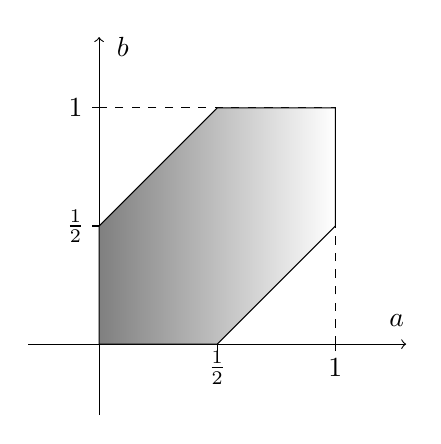
\begin{tikzpicture}[scale=3]
    \draw[->] (-0.3,0) -- (1.3,0) node at (1.26,0.1) {$a$};
    \draw[->] (0,-0.3) -- (0,1.3) node at (0.1,1.26) {$b$};;
    \draw (1,-0.03) -- (1,0.03);
    \draw (-0.03,1) -- (0.03,1);
    \draw (0.5,-0.03) -- (0.5,0.03);
    \draw (-0.03,0.5) -- (0.03,0.5);
    \draw[dashed] (1,0) -- (1,1) -- (0,1);
    \node at (1,-0.1) {$1$};
    \node at (-0.1,1) {$1$};
    \node at (0.5,-0.1) {$\frac{1}{2}$};
    \node at (-0.1,0.5) {$\frac{1}{2}$};
    \shadedraw[left color=gray,right color=white]  (0,0) -- (0.5,0) -- (1,0.5) -- (1,1) -- (0.5,1) -- (0,0.5) -- (0,0);
    \end{tikzpicture}
    \end{figure}
    Introducing the 3rd dimension, $|a-b|<\frac{1}{2}$ turns out to be an hexagonal prism (the base is shown above) whose height is 1 (along the c-axis). Similarly $|b-c| <\frac{1}{2}$ is the same solid, but rotated 90 degrees around the line parallel to the b-axis and going through the point($\frac{1}{2}$,$\frac{1}{2}$,$0$). Let's now compute the intersection between those solids, which turns out to be the sum of few smaller solids, in particular: 2 cubes with side $\frac{1}{2}$, 2 square pyramids with base length and height $\frac{1}{2}$ and 4 triangular prism, having height $\frac{1}{2}$ and an isosceles right triangle with side $\frac{1}{2}$ as base. Finally  the probability is $$\displaystyle p=\frac{2\cdot\frac{1}{8}+2\cdot\frac{1}{24}+4\cdot\frac{1}{8}}{1}=\frac{7}{12}$$ which leads to 712 as final answer.
\end{solution}\bigskip

        \newpage
            
		
\end{document}